\documentclass[a4paper, 12pt, twoside]{article}


%------------------------------------------------------------------------
%
% Author                :   arcln production
% Last modification     :   2023.1.12
%
%------------------------------------------------------------------------


%------ini
\usepackage[utf8]{inputenc}
\usepackage[T1]{fontenc}
\usepackage[french]{babel}
%\usepackage[english]{babel}
\usepackage{setspace}


%------geometry
\usepackage[textheight=700pt, textwidth=500pt]{geometry}


%------color
\usepackage{xcolor}
\definecolor{0010A1}{HTML}{0010A1}
\definecolor{00f}{HTML}{0000ff}
\definecolor{0ff}{HTML}{00ffff}
\definecolor{656565}{HTML}{656565}

%\renewcommand{\emph}{\textcolor{0010A1}}
%\renewcommand{\em}{\color{0010A1}}

\newcommand{\Emph}{\textcolor{0010A1}}

\newcommand{\strong}[1]{\textcolor{0010A1}{\bf #1}}
\newcommand{\st}{\color{0010A1}\bf}


%------Code highlighting
%---listings
\usepackage{listings}

\definecolor{cbg}{HTML}{272822}
\definecolor{cfg}{HTML}{ececec}
\definecolor{ccomment}{HTML}{686c58}
\definecolor{ckw}{HTML}{f92672}
\definecolor{cstring}{HTML}{e6db72}
\definecolor{cstringlight}{HTML}{98980f}
\definecolor{lightwhite}{HTML}{fafafa}

\lstdefinestyle{DarkCodeStyle}{
    backgroundcolor=\color{cbg},
    commentstyle=\itshape\color{ccomment},
    keywordstyle=\color{ckw},
    numberstyle=\tiny\color{cbg},
    stringstyle=\color{cstring},
    basicstyle=\ttfamily\footnotesize\color{cfg},
    breakatwhitespace=false,
    breaklines=true,
    captionpos=b,
    keepspaces=true,
    numbers=left,
    numbersep=5pt,
    showspaces=false,
    showstringspaces=false,
    showtabs=false,
    tabsize=4,
    xleftmargin=\leftskip
}

\lstdefinestyle{LightCodeStyle}{
    backgroundcolor=\color{lightwhite},
    commentstyle=\itshape\color{ccomment},
    keywordstyle=\color{ckw},
    numberstyle=\tiny\color{cbg},
    stringstyle=\color{cstringlight},
    basicstyle=\ttfamily\footnotesize\color{cbg},
    breakatwhitespace=false,
    breaklines=true,
    captionpos=b,
    keepspaces=true,
    numbers=left,
    numbersep=10pt,
    showspaces=false,
    showstringspaces=false,
    showtabs=false,
    tabsize=4,
    frame=L,
    xleftmargin=\leftskip
}

%\lstset{style=DarkCodeStyle}
\lstset{style=LightCodeStyle}
%Usage : \begin{lstlisting}[language=Caml, xleftmargin=xpt] ... \end{lstlisting}


%---Algorithm
\usepackage[linesnumbered,ruled,vlined]{algorithm2e}
\SetKwInput{KwInput}{Input}
\SetKwInput{KwOutput}{Output}

\SetKwProg{Fn}{Function}{:}{}
\SetKw{KwPrint}{Print}

\newcommand\commfont[1]{\textit{\texttt{\textcolor{656565}{#1}}}}
\SetCommentSty{commfont}
\SetProgSty{texttt}
\SetArgSty{textnormal}
\SetFuncArgSty{textnormal}
%\SetProgArgSty{texttt}

\newenvironment{indalgo}[2][H]{
    \begin{algoBox}
        \begin{algorithm}[#1]
            \caption{#2}
}
{
        \end{algorithm}
    \end{algoBox}
}


%---tcolorbox
\usepackage[many]{tcolorbox}
\DeclareTColorBox{emphBox}{O{black}O{lightwhite}}{
    breakable,
    outer arc=0pt,
    arc=0pt,
    top=0pt,
    toprule=-.5pt,
    right=0pt,
    rightrule=-.5pt,
    bottom=0pt,
    bottomrule=-.5pt,
    colframe=#1,
    colback=#2,
    enlarge left by=10pt,
    width=\linewidth-\leftskip-10pt,
}

\DeclareTColorBox{algoBox}{O{black}O{lightwhite}}{
    breakable,
    arc=0pt,
    top=0pt,
    toprule=-.5pt,
    right=0pt,
    rightrule=-.5pt,
    bottom=0pt,
    bottomrule=-.5pt,
    left=0pt,
    leftrule=-.5pt,
    colframe=#1,
    colback=#2,
    width=\linewidth-\leftskip-10pt,
}


%-------make the table of content clickable
\usepackage{hyperref}
\hypersetup{
    colorlinks,
    citecolor=black,
    filecolor=black,
    linkcolor=black,
    urlcolor=black
}


%------pictures
\usepackage{graphicx}
%\usepackage{wrapfig}

\usepackage{tikz}
%\usetikzlibrary{babel}             %Uncomment this to use circuitikz
%\usetikzlibrary{shapes.geometric}  % To draw triangles in trees
%\usepackage{circuitikz}            %Electrical circuits drawing


%------tabular
%\usepackage{color}
%\usepackage{colortbl}
%\usepackage{multirow}


%------Mathpartir (inference rules)
\usepackage{mathpartir}


%------Physics
%---Packages
%\usepackage[version=4]{mhchem} %$\ce{NO4^2-}$

%---Commands
\newcommand{\link}[2]{\mathrm{#1} \! - \! \mathrm{#2}}
\newcommand{\pt}[1]{\cdot 10^{#1}} % Power of ten
\newcommand{\dt}[2][t]{\dfrac{\mathrm d #2}{\mathrm d #1}} % Derivative


%------math
%---Packages
%\usepackage{textcomp}
%\usepackage{amsmath}
\usepackage{amssymb}
\usepackage{mathtools} % For abs
\usepackage{stmaryrd} %for \llbracket and \rrbracket
\usepackage{mathrsfs} %for \mathscr{x} (different from \mathcal{x})

%---Commands
%-Sets
\newcommand{\N}{\mathbb{N}} %set N
\newcommand{\Z}{\mathbb{Z}} %set Z
\newcommand{\Q}{\mathbb{Q}} %set Q
\newcommand{\R}{\mathbb{R}} %set R
\newcommand{\C}{\mathbb{C}} %set C
\newcommand{\U}{\mathbb{U}} %set U
\newcommand{\seg}[2]{\left[ #1\ ;\ #2 \right]}
\newcommand{\nset}[2]{\left\llbracket #1\ ;\ #2 \right\rrbracket}

%-Exponantial / complexs
\newcommand{\e}{\mathrm{e}}
\newcommand{\cj}[1]{\overline{#1}} %overline for the conjugate.

%-Vectors
\newcommand{\vect}{\overrightarrow}
\newcommand{\veco}[3]{\displaystyle \vect{#1}\binom{#2}{#3}} %vector + coord

%-Limits
\newcommand{\lm}[2][{}]{\lim\limits_{\substack{#2 \\ #1}}} %$\lm{x \to a} f$ or $\lm[x < a]{x \to a} f$
\newcommand{\Lm}[3][{}]{\lm[#1]{#2} \left( #3 \right)} %$\Lm{x \to a}{f}$ or $\Lm[x < a]{x \to a}{f}$
\newcommand{\tendsto}[1]{\xrightarrow[#1]{}}

%-Integral
\newcommand{\dint}[4][x]{\displaystyle \int_{#2}^{#3} #4 \mathrm{d} #1} %$\dint{a}{b}{f(x)}$ or $\dint[t]{a}{b}{f(t)}$

%-left right
\newcommand{\lr}[1]{\left( #1 \right)}
\newcommand{\lrb}[1]{\left[ #1 \right]}
\newcommand{\lrbb}[1]{\left\llbracket #1 \right\rrbracket}
\newcommand{\set}[1]{\left\{ #1 \right\}}
\newcommand{\abs}[1]{\left\lvert #1 \right\rvert}
\newcommand{\ceil}[1]{\left\lceil #1 \right\rceil}
\newcommand{\floor}[1]{\left\lfloor #1 \right\rfloor}
\newcommand{\lrangle}[1]{\left\langle #1 \right\rangle}

%-Others
\newcommand{\para}{\ /\!/\ } %//
\newcommand{\ssi}{\ \Leftrightarrow \ }
\newcommand{\eqsys}[2]{\begin{cases} #1 \\ #2 \end{cases}}

\newcommand{\med}[2]{\mathrm{med} \left[ #1\ ;\ #2 \right]}  %$\med{A}{B} -> med[A ; B]$
\newcommand{\Circ}[2]{\mathscr{C}_{#1, #2}}

\renewcommand{\le}{\leqslant}
\renewcommand{\ge}{\geqslant}

\newcommand{\oboxed}[1]{\textcolor{0010A1}{\boxed{\textcolor{black}{#1}}}} %orange boxed

\newcommand{\rboxed}[1]{\begin{array}{|c} \hline #1 \\ \hline \end{array}} %boxed with right opened
\newcommand{\lboxed}[1]{\begin{array}{c|} \hline #1 \\ \hline \end{array}} %boxed with left opened

\newcommand{\orboxed}[1]{\textcolor{0010A1}{\rboxed{\textcolor{black}{#1}}}} %orange right boxed
\newcommand{\olboxed}[1]{\textcolor{0010A1}{\lboxed{\textcolor{black}{#1}}}} %orange left boxed


%------commands
%---to quote
\newcommand{\simplecit}[1]{\guillemotleft$\;$#1$\;$\guillemotright}
\newcommand{\cit}[1]{\simplecit{\textcolor{656565}{#1}}}
\newcommand{\quo}[1]{\cit{\it #1}}

%---to indent
\newcommand{\ind}[1][20pt]{\advance\leftskip + #1}
\newcommand{\deind}[1][20pt]{\advance\leftskip - #1}

%---to indent a text
\newcommand{\indented}[2][20pt]{\par \ind[#1] #2 \par \deind[#1]}
\newenvironment{indt}[2][20pt]{#2 \par \ind[#1]}{\par \deind} %Titled indented env

%---title
\newcommand{\thetitle}[2]{\begin{center}\textbf{{\LARGE \underline{\Emph{#1} :}} {\Large #2}}\end{center}}

%---Maths environments
%-Proofs
\newenvironment{proof}[1][{}]{\begin{indt}{$\square$ #1}}{$\blacksquare$ \end{indt}}

%-Maths parts (proposition, definition, ...)
\newenvironment{mathpart}[1]{\begin{indt}{\boxed{\text{\textbf{#1}}}}}{\end{indt}}
\newenvironment{mathbox}[1]{\boxed{\text{\textbf{#1}}}\begin{emphBox}}{\end{emphBox}}
\newenvironment{mathul}[1]{\begin{indt}{\underline{\textbf{#1}}}}{\end{indt}}

\newenvironment{theo}{\begin{mathpart}{Théorème}}{\end{mathpart}}
\newenvironment{Theo}{\begin{mathbox}{Théorème}}{\end{mathbox}}

\newenvironment{prop}{\begin{mathpart}{Proposition}}{\end{mathpart}}
\newenvironment{Prop}{\begin{mathbox}{Proposition}}{\end{mathbox}}
\newenvironment{props}{\begin{mathpart}{Propriétés}}{\end{mathpart}}

\newenvironment{defi}{\begin{mathpart}{Définition}}{\end{mathpart}}
\newenvironment{meth}{\begin{mathpart}{Méthode}}{\end{mathpart}}

\newenvironment{Rq}{\begin{mathul}{Remarque :}}{\end{mathul}}
\newenvironment{Rqs}{\begin{mathul}{Remarques :}}{\end{mathul}}

\newenvironment{Ex}{\begin{mathul}{Exemple :}}{\end{mathul}}
\newenvironment{Exs}{\begin{mathul}{Exemples :}}{\end{mathul}}


%------Sections
% To change section numbering :
% \renewcommand\thesection{\Roman{section}}
% \renewcommand\thesubsection{\arabic{subsection})}
% \renewcommand\thesubsubsection{\textit \alph{subsubsection})}

% To start numbering from 0
% \setcounter{section}{-1}


%------page style
\usepackage{fancyhdr}
\usepackage{lastpage}

\setlength{\headheight}{18pt}
\setlength{\footskip}{50pt}

\pagestyle{fancy}
\fancyhf{}
\fancyhead[LE, RO]{\textit{\textcolor{black}{\today}}}
\fancyhead[RE, LO]{\large{\textsl{\Emph{\texttt{Rapport de Projet}}}}}

\fancyfoot[RO, LE]{\textit{\texttt{\textcolor{black}{Page \thepage /}\pageref{LastPage}}}}
\fancyfoot[LO, RE]{
\includegraphics[scale=0.12]{arcln}}


%------init lengths
\setlength{\parindent}{0pt} %To avoid using \noindent everywhere.
\setlength{\parskip}{3pt}

% Mise en page française
\usepackage[utf8]{inputenc}
\usepackage[french]{babel}
\usepackage{geometry}

% Import d'images, couleurs
\usepackage{graphicx,color}

\usepackage{lipsum}

\newcommand{\hsp}{\hspace{20pt}}
\newcommand{\HRule}{\rule{\linewidth}{0.5mm}}
\onehalfspacing

%---------------------------------Begin Document
\begin{document}

    
\begin{titlepage}
  \begin{sffamily}
  \begin{center}

  
    
\includegraphics[scale=0.3]{logo}~\\[1.5cm]

    \textsc{\LARGE EPITA Rennes}\\[0.5cm]

    % Titre
    \textsc{\Large RAPPORT DU PROJET S2}\\[1.5cm]

    \HRule \\[0.4cm]
     { \huge \bfseries  A Slime's Journey \\[0.4cm] }

    \HRule \\[2cm]
    
\includegraphics[scale=0.4]{arcln}
     \\[0.5cm]
    %\textsc{\Large ARCLN}\\[1.5cm]

    % Membres
    \begin{minipage}{0.4\textwidth}
      \begin{flushleft} \large
        Alexis LE GALL\\
        Enzo JUHEL\\
      \end{flushleft}
    \end{minipage}
    \begin{minipage}{0.4\textwidth}
      \begin{flushright} \large
        Maxime DOUILLARD\\
        Omid SHEIBANIFAR\\
      \end{flushright}
    \end{minipage}

    \vfill

  \end{center}
  \end{sffamily}
\end{titlepage}


    \tableofcontents
    \newpage

    \begin{indt}{\section{Introduction}}
        En cette fin d’année d'enseignement supérieur à l’Epita de Rennes (35), nous avons rédigé ce document dans lequel vous prendrez connaissances des différentes étapes du développement ainsi que la chronologie des avancées de chacuns, restituées personnellement.

        Ce rapport est réalisé dans le cadre du projet semestre deux de l’école. Les membres Alexis Le Gall, Enzo Juhel, Omid Sheibanifar et Maxime Douillard, représentant la structure ARCLN prod, ont créé le jeu “A Slime’s Journey”. C’est un platformer 2D se déroulant à l’époque médiévale, dont la difficulté croît avec l’évolution du ou des personnages.

        Chaque joueur prend le contrôle d'un slime virtuel :

        Un monstre imaginaire visqueux de morphologie minimaliste, sorte de blob vert obligé de se déplacer, par rebond, d’avant en arrière dans un décor médiéval.

        \begin{figure}[h]
            \centering
            
\includegraphics[width=0.5\textwidth]{logo.png}
            \caption{Le Slime}
            \label{fig:mesh1}
        \end{figure}

        Afin d’évoluer dans l’aventure, il doit atteindre d’autres plateformes mais aussi attaquer des ennemies en leur sautant dessus.

        C’est dans un univers pixelisé du Moyen- ge qu’une coopération à deux en ligne est possible. En effet, cette option rend le jeu plus convivial en partageant une entraide réelle tout au long de l’aventure.
        La fonction multijoueurs ne change en rien les niveaux de difficultés, ni le scénario parcouru.
        Chaque joueur prend la main sur son personnage avec des capacités de mouvements, d’attaques et de transformations physiques similaires, type roche ou type feu.

        Et pour finaliser ce rapport  une comparaison en rétrospective de ce que nous avions prévu pour cette soutenance finale, suivi de l’annexe comprenant les ressources utiles à la compréhension de l’avancée du projet est à disposition.
    \end{indt}

    \newpage

    \begin{indt}{\section{Résumé cahier des charges}}
        Pour ce projet, notre entreprise a décidé de créer un jeu de plateforme en 2D. Inspiré de divers jeux vidéo, notre jeu comportera certaines ressemblances avec eux mais aussi certains des points de divergences. Le joueur prendra le contrôle d'un slime, une sorte de blob qui peut se déplacer avec des petits sauts. En multijoueur, les joueurs pourront vaincre des monstres se trouvant sur leur passage à l'aide d'équipement ramassé au préalable durant les précédents niveaux, ou à l'aide de leurs capacités temporaires, qu’ils pourront acquérir sur le terrain en passant sur certains objets, comme une pierre, permettant d’accéder à la première transformation.

        \begin{center}
            \begin{tabular}{|c|c|c|c|c|}
                \hline
                & Alexis & Enzo & Maxime & Omid
                \\
                \hline
                Développement & Participant & Participant & Responsable & Suppléant
                \\
                \hline
                Communication & Suppléant & & Responsable &
                \\
                \hline
                Design & & Responsable & Suppléant &
                \\
                \hline
                Audio & Suppléant & & & Responsable
                \\
                \hline
                IA & Responsable & & & Suppléant
                \\
                \hline
                Réseau & Responsable & Suppléant & Participant & Participant
                \\
                \hline
                Rédaction & Participant & Responsable & Participant & Suppléant
                \\
                \hline
            \end{tabular}
        \end{center}
    \end{indt}

    \begin{indt}{\section{Chronologie des avancements personnels}}
        Lors de notre première soutenance, nous avons commencé par générer l'idée de notre jeu et avons élaboré un cahier des charges détaillé.De plus, nous avons créé le premier niveau du jeu, en mettant l'accent sur une expérience multijoueur immersive. Pour rendre le gameplay plus intéressant, nous avons introduit un premier ennemi, le sanglier qui offre des défis aux joueurs. De plus, nous avons mis en place un menu principal convivial pour faciliter la navigation dans le jeu.
        Notre deuxième soutenance a été marquée par l'ajout du deuxième niveau, offrant ainsi une progression plus riche pour les joueurs. Nous avons également introduit la transformation du slime sous forme de roche avec un sprite unique et un système d'escalade pour ajouter une dimension supplémentaire au gameplay. De plus, nous avons développé un prototype de projectile, permettant aux joueurs de lancer des attaques à distance. Pour rendre l'expérience encore plus captivante, nous avons inclus des pièges dans le jeu, créant ainsi des obstacles supplémentaires. De nouveaux adversaires, tels que les villageois et les archers, ont également été intégrés pour enrichir les combats.
        Lors de notre dernière soutenance, nous avons décidé d’éradiquer les bugs restants et avons franchi une étape majeure en introduisant un boss puissant qui représente un défi ultime pour les joueurs. Nous avons également ajouté une nouvelle forme du slime, comprenant des flammes, avec son propre sprite et des projectiles associés, apportant une diversité d'attaques et de stratégies. Pour améliorer l'expérience utilisateur, nous avons inclus des options dans le jeu, notamment la personnalisation des touches, les réglages de résolution et de volume. Ces fonctionnalités permettent aux joueurs de personnaliser leur expérience de jeu selon leurs préférences.
        Ces trois soutenances ont été essentielles pour le développement de notre jeu. Chaque étape a apporté de nouvelles fonctionnalités, des défis supplémentaires et des améliorations générales pour offrir une expérience de jeu immersive et engageante. Grâce à notre travail acharné et à notre progression étape par étape, nous avons pu créer un jeu plus complexe, offrant une diversité de niveaux, de monstres et de fonctionnalités pour le plus grand plaisir des joueurs.

        \begin{indt}{\subsection{Omid}}
            \begin{figure}[h]
                \centering
                
\includegraphics[width=0.5\textwidth]{omid.png}
                \caption{Omid}
                \label{fig:mesh1}
            \end{figure}

            Après la seconde soutenance, nous nous sommes tout d’abord mit à régler les nombreux bugs que ce soit au niveau de la synchronisation en multijoueur, ou des textures du niveau 2 ou encore des animations et transformations. Après cela, j’ai continué à perfectionner les animations du slime et des ennemis avec notamment des animations de dégâts dans des cas précis comme par exemple lorsque le slime est en mode roche, qu’il saute et qu’il prend des dégâts. J’ai aussi travaillé sur l’animation de la transformation de feu et fait en sorte de pouvoir se transformer grâce au feu de camp.

            Par la suite, j’ai créé une pomme permettant au joueur de regagner une vie s' il en avait perdu.

            De plus, j’ai ajouté des sons de morts aux ennemis qui n’en avaient pas et créé un système d’effets sonores lorsque le joueur arrive dans une certaine zone.

            Enfin, je me suis chargé de créer notre premier boss: le bûcheron. Ce dernier ayant plusieurs attaques et plusieurs phases, est l’IA la plus développée de notre jeu (voir partie IA pour plus d’informations sur le bucheron).
        \end{indt}

        \begin{indt}{\subsection{Alexis}}
            \begin{figure}[h]
                \centering
                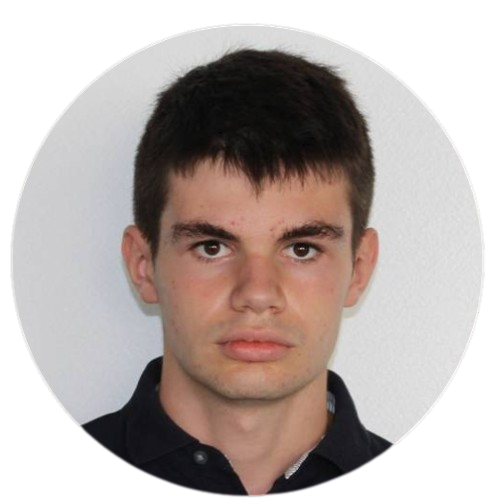
\includegraphics[width=0.5\textwidth]{alexis.png}
                \caption{Alexis}
                \label{fig:mesh1}
            \end{figure}

            Suite à la soutenance technique, notre équipe s'est concentrée sur la résolution de nombreux problèmes, que ce soit au niveau de la synchronisation en multijoueur, des textures du niveau 2 ou encore des animations et des transformations. Une fois ces problèmes résolus, j'ai poursuivi mes efforts pour améliorer les animations du slime et des ennemis. J'ai notamment travaillé sur des animations de dégâts spécifiques, comme lorsque le slime est en mode roche, qu'il saute et qu'il subit des dommages.

            Mon objectif était de rendre ces animations plus fluides et réactives, afin d'améliorer l'expérience globale du jeu. J’ai confectionné les sprites des différentes transformations et rajouté des sprites pour les situations spécifiques aux transformations.

        \end{indt}

        \newpage

        \begin{indt}{\subsection{Enzo}}
            \begin{figure}[h]
                \centering
                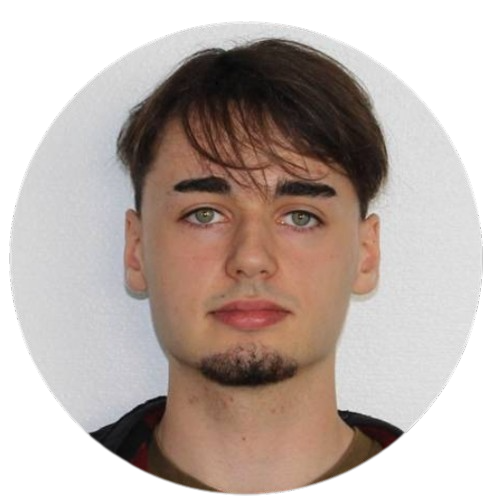
\includegraphics[width=0.5\textwidth]{enzo.png}
                \caption{Enzo}
                \label{fig:mesh1}
            \end{figure}

            Dès la fin de la seconde soutenance, j'ai concentré mes efforts sur la résolution des problèmes majeurs qui affectaient la jouabilité du jeu. L'un de ces problèmes était lié à la synchronisation en multijoueur, en particulier lors de la réapparition d'un joueur et du passage au deuxième niveau. J'ai travaillé sur ces bugs pour éviter la disparition d'un joueur ou de tous les monstres lors de ces transitions. Grâce à mes efforts, ces problèmes ont été résolus, permettant ainsi aux joueurs de profiter d'une expérience multijoueur plus fluide et sans dysfonctionnements.

            En plus de la résolution des bugs, j'ai apporté de nombreuses améliorations et nouveautés au jeu. J'ai implémenté un menu permettant aux joueurs de personnaliser les touches utilisées en jeu, offrant ainsi une plus grande flexibilité et adaptabilité aux préférences de chacun. De plus, j'ai ajouté un indicateur visuel pour signaler au joueur quand il a la possibilité de se transformer, et cet indicateur s'ajuste automatiquement en fonction des touches configurées par l'utilisateur, assurant ainsi une expérience de jeu intuitive et personnalisée.

            J'ai également travaillé sur l'aspect visuel et l'interface du jeu. J'ai créé un écran de transition fluide entre chaque changement de scène, offrant une transition visuelle agréable et cohérente. J'ai déplacé la position des cœurs affichant la santé du personnage en haut à gauche de l'écran, offrant une disposition plus ergonomique et permettant aux joueurs de garder un œil sur leur état de santé plus facilement pendant le jeu. De plus, j'ai ajouté l'affichage du nom de la partie en cours en bas à gauche de l'écran, facilitant ainsi la communication entre les joueurs lors d'une session multijoueur.

            En ce qui concerne les animations du slime, j'ai créé un nouveau sprite représentant le slime de roche en train de sauter, ainsi qu'un sprite montrant le slime de roche subissant une attaque. Ces animations ajoutent du dynamisme et de la vie au personnage principal, renforçant ainsi l'immersion et l'expérience visuelle du joueur.

            Grâce à ces avancées et améliorations, j'ai contribué à rendre "A Slime's Journey" plus stable, plus convivial et plus agréable pour les joueurs. Ces améliorations tant au niveau des fonctionnalités que de l'aspect visuel ont permis de renforcer l'expérience globale du jeu, offrant aux joueurs une expérience plus fluide, immersive et engageante.

        \end{indt}

        \begin{indt}{\subsection{Maxime}}
            \begin{figure}[h]
                \centering
                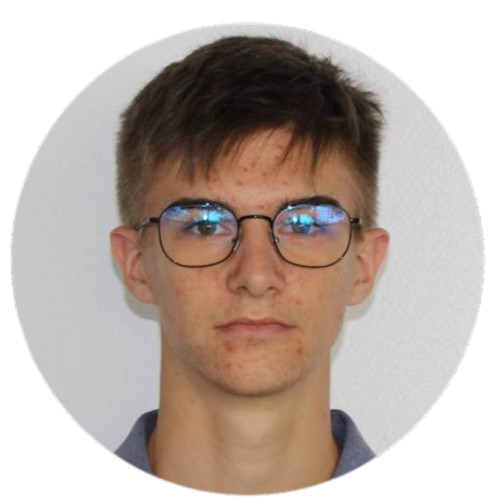
\includegraphics[width=0.5\textwidth]{maxime.png}
                \caption{Maxime}
                \label{fig:mesh1}
            \end{figure}

            Suite à cette soutenance, nous avons pris la décision d’un commun accord qu’il fallait en priorité éradiquer les bugs existants, ainsi que de commencer à implémenter certaines fonctionnalités qui permettront au joueur d’avoir un meilleur confort de jeu et rendre ainsi l’expérience de jeu plus plaisante. J’ai commencé par implémenter une première version de personnalisation de touches que nous n’avons pas gardé par question de simplicité.

            J’ai également été chargé de réaliser un menu d’options permettant de changer la résolution du jeu, ainsi que le volume dans le jeu.

            Ce projet m’a fait réaliser à quel point il peut être plaisant de réaliser un jeu vidéo de A à Z.
        \end{indt}
    \end{indt}

    \newpage

    \begin{indt}{\section{Avance / Retard}}
        Le développement du jeu vidéo "A Slime's Journey" a été un voyage ponctué d'avancées passionnantes et de défis inattendus. Nous avons investi énormément de temps et d'efforts dans ce projet, et bien que nous ayons rencontré des retards par rapport à notre cahier des charges initial, chaque étape a été l'occasion d'apprendre et de grandir. Malheureusement, le mode versus, qui aurait ajouté une dimension compétitive captivante, ainsi que le mode boss rush, avec ses affrontements palpitants contre plusieurs boss, n'ont pas pu être intégrés tels que prévus. Nous avons dû faire face à des contraintes de temps et de ressources qui nous ont obligés à revoir nos priorités. De plus, l'absence d'un troisième niveau dans le jeu a été une déception, mais cela n'a pas entaché l'intérêt et le plaisir que procure l'expérience de jeu. Malgré ces ajustements, nous sommes fiers du résultat obtenu. Chaque bug corrigé, chaque fonctionnalité implémentée représente une victoire pour notre équipe. Nous avons relevé le défi de travailler avec l'API Photon pour la première fois, ce qui a nécessité une veille technique constante et une volonté d'apprendre en permanence. Ce projet a également été notre première expérience de longue durée, nous confrontant à des situations inattendues qui ont renforcé notre capacité à travailler en équipe et à surmonter les obstacles. Le jeu "A Slime's Journey" est le fruit d'une collaboration passionnée, et bien que nous ayons dû faire des compromis, nous sommes convaincus que nous avons créé une expérience de jeu intéressante qui saura captiver les joueurs.
    \end{indt}

    \begin{indt}{\section{Etat de l’art}}
        L'évolution des jeux de plate-forme a connu une riche histoire depuis leurs débuts dans les années 1980. Le genre a commencé avec des titres tels que Space Panic en 1980, qui n'autorisait pas les sauts, mais a ouvert la voie à l'innovation. Cependant, c'est le légendaire jeu Donkey Kong de Nintendo sorti en 1981 qui a introduit la mécanique de saut, devenant ainsi le premier véritable jeu de plate-forme. À partir de 1982, une multitude de jeux de plate-forme ont vu le jour, notamment Pitfall, Manic Miner, Jet Set Willy, Impossible Mission et Prince of Persia. Cependant, c'est en 1985 que le jeu révolutionnaire "Super Mario Bros" est apparu, devenant un énorme succès avec plus de 40 millions d'exemplaires vendus. Il a établi les normes du genre grâce à sa jouabilité intuitive et sa capacité à offrir une expérience de jeu captivante. Par la suite, le genre a évolué vers des jeux en 3D, avec l'emblématique Super Mario 64 en 1996. Depuis lors, les jeux de plate-forme continuent de prospérer, avec des titres tels que Super Meat Boy en 2010, de nouveaux opus de la série "Super Mario Bros" et bien d'autres. L'état de l'art des jeux de plate-forme témoigne de leur durabilité et de leur capacité à captiver les joueurs au fil des décennies.

        \begin{figure}[h]
            \centering
            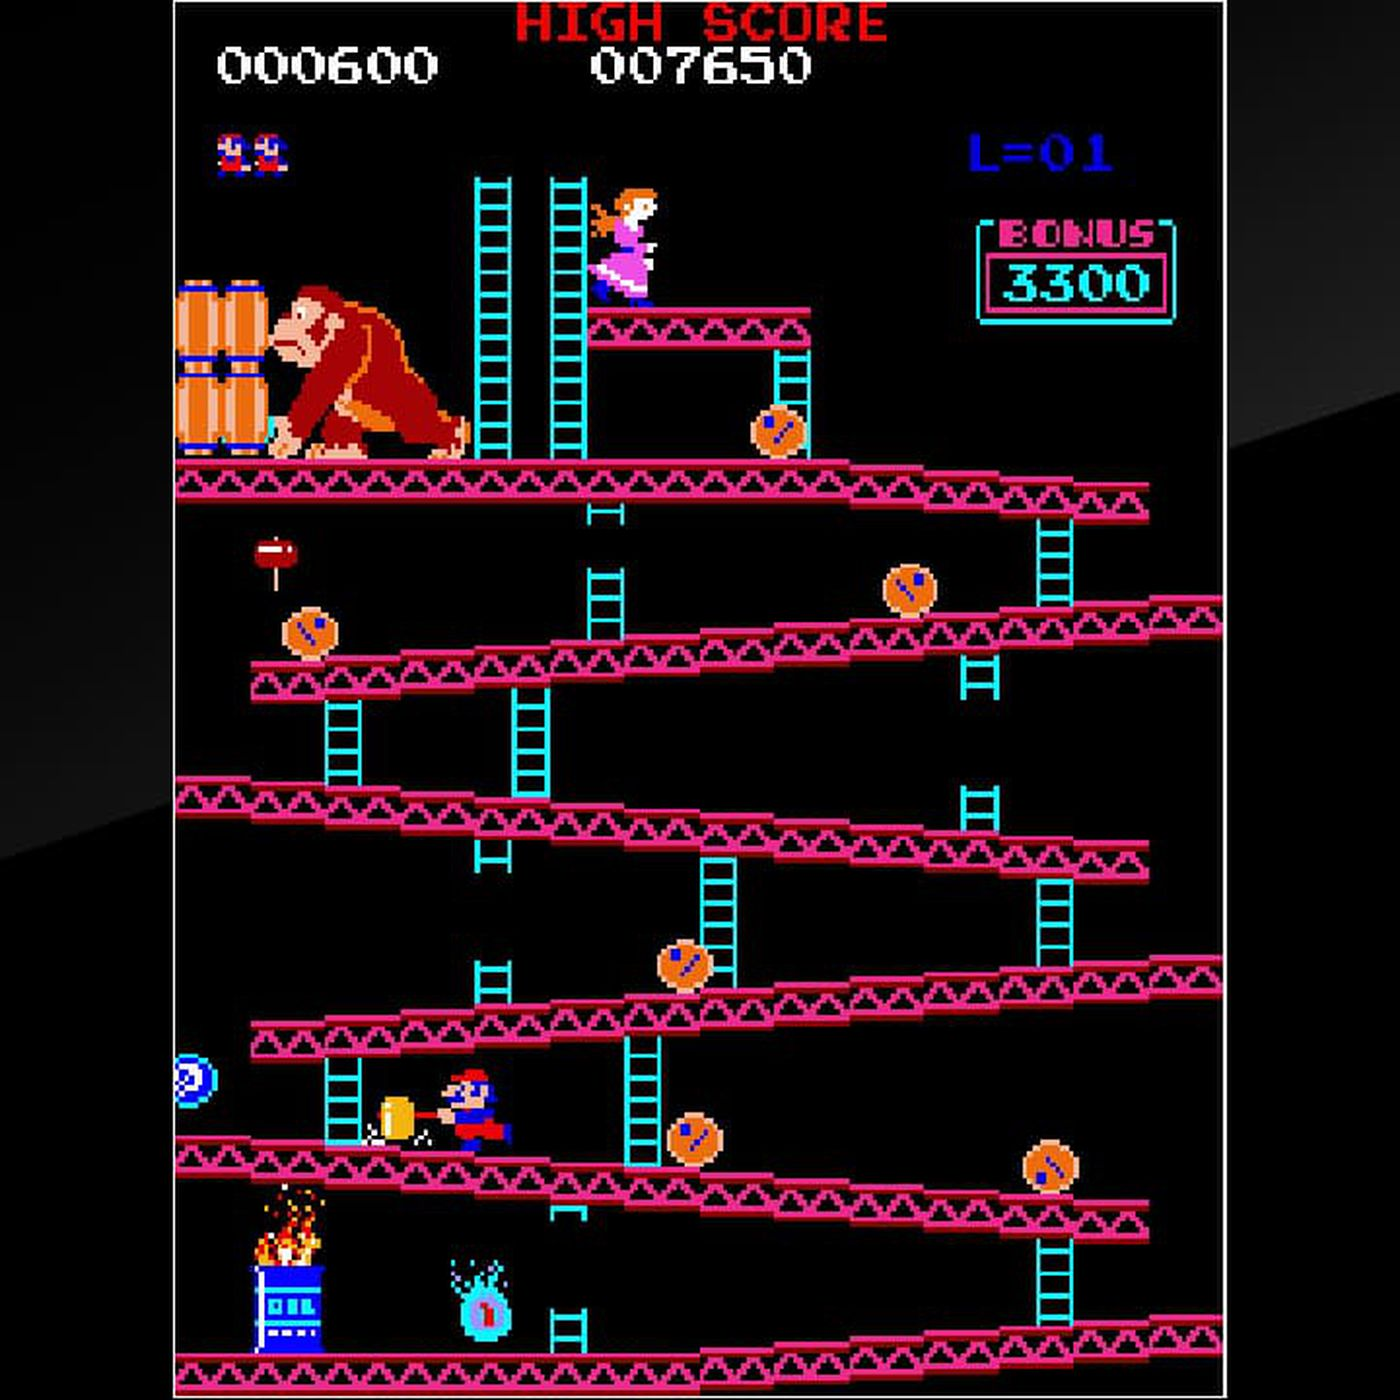
\includegraphics[width=0.6\textwidth]{SMB2.jpg}
            \caption{Donkey Kong}
            \label{fig:mesh1}
        \end{figure}
    \end{indt}

    \newpage

    \begin{indt}{\section{Origine}}
        Ayant tous joué à des jeux de plateformes 2D durant notre enfance, tel que "Super Mario Bros", il s'est avéré que c'était un type de jeu que nous connaissons tous très bien et avec de nombreuses références permettant une maîtrise du sujet. De plus, une créature fantastique simple mais au caractère divers, le slime, nous a paru une évidence d'où sa place de héros dans le jeu, sans oublier que les power up, l'exploration, les combats, etc font partie de l'univers des jeux vidéo et permettent un niveau d'immersion supérieur. D'ailleurs un autre aspect des jeux vidéos sont leur univers, mieux ceux-ci sont construit, mieux le joueur va s'y retrouver immergé, pour cela, nous avons pris la liberté de construire un univers, une histoire et une intrigue se développant tout au long des différents niveaux et qui sera assimilable par le joueur au travers de l'aspect d'exploration du jeu. C'est ainsi que nous avons donc décidé de partir sur ce modèle de jeu vidéo, un simple platformer 2D renfermant une histoire profonde répartie sur plusieurs niveaux.
    \end{indt}


    \begin{indt}{\section{Rapport des avancées}}
        La prise en mains de Unity 3D à été un peu compliquée au début mais nous nous sommes vite habitué et grâce aux nombreux tutoriels disponibles sur internet, sous la forme de cours ou de vidéo. De plus, l'ensemble des scripts utilisés par ce moteur ont été programmé en C$\#$ avec Visual Studio Code et Rider grâce au Développer Pack du .NET Framework 4.7.1.

        La mise en place du site web fut difficile quant à la mise en place du site internet.

        Depuis, nous avons effectué une refonte visuelle du premier niveau. De plus, nous avons également décidé d’ajouter une option afin de réapparaître après la mort d’un joueur. De nombreux bugs ont été réparés, tournant en partie autour de la synchronisation du multijoueur, qui pouvait causer des surcharges de la mémoire et par conséquent mettre à mal la partie en cours.

        De plus, nous avons également ajouté un menu permettant au joueur d'associer lui-même les touches permettant d’effectuer les actions, lui donnant ainsi plus de liberté et de confort de jeu.

        Pour continuer sur le confort de jeu, nous avons également rendu la création de partie multijoueur insensible à la casse, nous pouvons désormais écrire avec où sans majuscule, la partie rejoint sera la même.

        \newpage

        \begin{indt}{\subsection{Graphismes}}
            Dans "A Slime's Journey", nous avons pris la décision de maintenir une direction artistique cohérente en optant pour un style pixelisé, qui renvoie aux origines même des jeux vidéo. Ce choix est motivé par notre volonté de rappeler l'essence des anciens jeux de plateformes, tout en rendant hommage à des titres plus récents qui ont également adopté ce style rétro, tels que le célèbre jeu "Céleste".

            \begin{figure}[h]
                \centering
                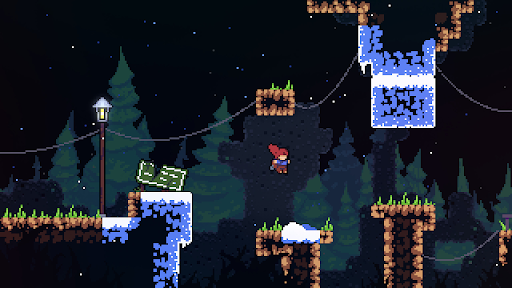
\includegraphics[width=0.6\textwidth]{Celeste.png}
                \caption{Céleste}
                \label{fig:mesh1}
            \end{figure}

            Les graphismes pixelisés offrent une esthétique charmante et nostalgique, faisant appel aux souvenirs des joueurs les plus passionnés. Chaque élément visuel du jeu, des décors aux personnages, est soigneusement conçu pour évoquer l'esprit des classiques des jeux de plateformes. Les pixels donnent une sensation d'authenticité et contribuent à créer une atmosphère immersive qui transporte les joueurs dans un monde rétro-futuriste captivant.

            En optant pour ce style, nous souhaitons également mettre en avant le gameplay et l'expérience de jeu. Les graphismes pixelisés permettent une lisibilité claire des plateformes, des obstacles et des ennemis, facilitant ainsi la navigation et la prise en main du jeu. De plus, ce style artistique nous offre une grande flexibilité dans la conception des niveaux et des environnements, nous permettant de créer des mondes variés et imaginatifs tout en restant fidèles à notre vision initiale.

            L'inspiration que nous tirons de jeux comme "Céleste" se manifeste dans notre attention portée aux détails et à la fluidité des animations. Chaque mouvement du slime, chaque interaction avec les ennemis ou les objets est soigneusement animé pour offrir une expérience de jeu fluide et agréable. Nous nous efforçons de créer un monde visuellement attrayant, où les joueurs seront transportés par les visuels rétro tout en étant immergés dans une aventure captivante et pleine de rebondissements.

            En résumé, notre décision de maintenir le style pixelisé dans les graphismes de "A Slime's Journey" est le fruit d'une volonté de rappeler l'essence des jeux de plateformes classiques tout en rendant hommage à des titres contemporains qui ont également embrassé ce style rétro. Les graphismes pixelisés apportent une touche nostalgique, tout en offrant une lisibilité claire et une expérience de jeu fluide. Ils contribuent à créer un univers visuel cohérent et immersif qui fera voyager les joueurs à travers une aventure inoubliable.
        \end{indt}

        \begin{indt}{\subsection{Les Logos}}
            Notre logo est resté le même depuis la première soutenance, en effet, il représente notre groupe depuis le début, et le logo nous plaisant à tous les 4, nous n’avons pas de raison de le changer, puisqu’il est sobre mais esthétique aussi.

            Dans notre logo pour "A Slime's Journey", nous avons opté pour une représentation unique et distinctive. Au centre du logo se trouve un graphique mathématique représentant une courbe exponentielle, symbolisant la progression et l'évolution constante dans le jeu. Cette courbe est stylisée de manière artistique, ajoutant une touche visuelle captivante à l'ensemble.

            Juste en dessous de la courbe exponentielle, nous avons placé le nom de notre équipe, ARCLN, dans une police de caractères audacieuse et claire. Cette mention permet d'identifier notre équipe de développement et de lui donner une présence forte dans le logo. Enfin, en bas du logo, nous avons ajouté le texte accrocheur "Nous ne brassons pas d'Euler", un jeu de mots qui souligne notre approche créative et notre passion pour le développement du jeu.

            L'utilisation de la courbe exponentielle dans notre logo représente non seulement la progression du joueur à travers les niveaux du jeu, mais aussi notre propre progression en tant qu'équipe de développement. Elle évoque également une sensation de mouvement et d'aventure, invitant les joueurs à se lancer dans une expérience immersive et stimulante.

            En combinant les éléments mathématiques, le nom de notre équipe et le jeu de mots astucieux, notre logo parvient à capturer l'essence de "A Slime's Journey" tout en offrant un design original et distinctif. Il est à la fois représentatif de notre jeu et de notre équipe, et nous sommes fiers de l'avoir choisi comme symbole visuel de notre projet.

            \begin{figure}[h]
                \centering
                
\includegraphics[width=0.25\textwidth]{Logo2.png}
                \caption{Logo du groupe}
                \label{fig:mesh1}
            \end{figure}

            Le logo que nous avons conçu met en valeur un slime vert. En choisissant un slime, nous souhaitons véhiculer un sentiment d’aventure, tout en rappelant la nostalgie des jeux rétro.

            \begin{figure}[h]
                \centering
                
\includegraphics[width=0.5\textwidth]{logo.png}
                \caption{Logo du jeu}
                \label{fig:mesh1}
            \end{figure}
        \end{indt}

        \newpage

        \begin{indt}{\subsection{Multijoueur}}
            L'un des aspects les plus importants du jeu "A Slime's Journey" est son mode multijoueur, qui a été implémenté dès le début du projet en utilisant l'extension Unity appelée Photon. Photon offre une API complète et permet l'hébergement gratuit des parties sur leurs serveurs. Au départ, nous avons suivi un tutoriel disponible sur le site de Photon, ce qui nous a permis de créer une première version du multijoueur où les joueurs pouvaient uniquement rejoindre des parties générées aléatoirement.

            Cependant, après une remise à zéro du projet, nous avons tous acquis une meilleure compréhension de l'API de Photon, ce qui nous a permis de réimplémenter de manière plus complète et sophistiquée le système de multijoueur. Cette nouvelle implémentation nous a donné la possibilité de créer et de rejoindre des parties en fonction de leur nom, offrant ainsi aux joueurs une expérience plus personnalisée et conviviale.

            Un des problèmes que nous avons résolus grâce à Photon était lié à l'instanciation des ennemis. Auparavant, les monstres apparaissaient localement pour chaque joueur, ce qui causait des incohérences dans le gameplay. En utilisant Photon, nous avons réussi à synchroniser l'instanciation des ennemis pour tous les joueurs, créant ainsi une expérience de jeu plus fluide et cohérente.

            Nous avons aussi réglé le problème de l’instantiation des projectiles par les joueurs qui ne sont pas hôtes de la partie, Tout d'abord, nous avons configuré les méthodes RPC nécessaires dans notre code de jeu. Nous avons créé une méthode RPC spécifique qui permet aux clients de demander l'instantiation d'un projectile sur le serveur. Cette méthode doit être appelée par les clients au moment de lancer un projectile.Lorsqu'un joueur effectue une action de lancement de projectile, nous avons utilisé les mécanismes fournis par Photon pour appeler la méthode RPC correspondante sur le serveur. Cela permettait de signaler au serveur qu'un projectile devait être instancié.

            De plus, grâce à l'implémentation du multijoueur avec Photon, nous avons pu résoudre un problème où la mort d'un joueur entraînait la mort de tous les joueurs de la partie. En synchronisant les événements de mort et les mécaniques de résurrection, nous avons créé un système robuste qui permet à chaque joueur de continuer à jouer indépendamment des actions des autres.

            Grâce à ces avancées dans le développement du multijoueur, "A Slime's Journey" offre désormais une expérience de jeu en ligne immersive et interactive. Les joueurs peuvent créer et rejoindre des parties spécifiques, collaborer avec leurs amis et affronter des défis ensemble. Cette dimension multijoueur ajoute une toute nouvelle dimension sociale et compétitive au jeu, offrant aux joueurs une expérience encore plus engageante et divertissante.

            En parlant de compétitivité, nous avons mis en place un chronomètre qui mesure le temps que prend un joueur pour finir le jeu (tous les niveaux). Au début du projet, nous avions envisagé de créer un mode versus permettant aux joueurs de s’affronter en un contre un. Cependant, nous avons pensé que cela s'éloignait trop de l’univers du jeu qui est un jeu de plateforme coopératif. Nous avons donc mis en place ce chronomètre placé en haut à droite de l’écran. Cela permet d’une part de donner aux joueurs le temps qu’ils ont mis pour finir le jeu et surtout de pouvoir défier leurs amis à battre leur score. Cela pousse le joueur à toujours essayer de s’améliorer afin de réaliser un meilleur temps que précédemment.

            Pour réaliser ce chronomètre, nous ajoutons à chaque frame passée le temps du jeu. Pour obtenir le temps en minutes on le divise par 60 (division entière) et pour les secondes on prend le reste de cette division.

        \end{indt}

        \begin{indt}{\subsection{Caméra}}
            La caméra fut un des éléments les plus embêtants à gérer et est d'ailleurs une des principales raisons pour lesquelles on a décidé de recommencer le projet le 3 Mars.

            Au début, nous avions fait en sorte que la caméra qui suit le joueur soit la caméra principale du jeu. Nous avions fait un script qui fait déplacer la caméra avec les déplacements du joueur. Cependant, même si cela marchait parfaitement en mode solo, en multijoueur la caméra principale n'arrivait pas à suivre les deux joueurs quand les deux bougeaient en même temps. Nous avons donc ensuite créé une caméra liée au joueur dans le dossier Ressources de Photon, créée en dehors de la scène du niveau. Cela permet de faire en sorte que chaque joueur ait sa propre caméra lorsque l'on lance le jeu. Théoriquement, cela aurait dû marcher parfaitement. Tout d'abord, la caméra suivait bien le joueur mais ne montrait rien. On a pu régler ce problème en reculant la caméra sur l'axe z. Ensuite, bien qu'en solo cela marche très bien, en multijoueur, les caméras des deux joueurs s'inversaient. En effet, le joueur déjà présent sur le niveau prenait la caméra du joueur qui avait rejoint et ce dernier prenait la caméra du joueur déjà présent.

            Ainsi, c'est à ce moment-là que nous avons décidé de recommencer le projet afin d'avoir un projet plus propre et de recommencer avec des bases solides. Lors de la première version, nous avions eu de nombreux problèmes avec la caméra, en effet, lors d'une partie en solitaire, le joueur avait bien la caméra réglée sur lui, qui la suivait correctement. Les problèmes arrivent lors d'une partie en multijoueurs, en effet, lorsque le premier joueur se connecte, il a sa propre caméra, mais, lorsqu'un second joueur se connecte, la caméra du joueur 1 va sur le joueur 2 et la caméra du joueur 2 va sur le joueur 1. Cela est dû au fait que la nouvelle instance de caméra essaye de se fixer sur le dernier joueur créer, ou alors de se fixer sur la première autre instance de joueur qu'il trouve sans caméra.

            Suite à notre incapacité à résoudre ce bug, nous avons décidé de recommencer le projet en partant de rien.

            C'est à partir de ce constat que nous avons ré-implémenté le multijoueur afin de régler ce bug majeur, et d'autres bugs mineurs liés au multijoueur. Cela étant fait, nous avons dû faire face à un autre bug de caméra, le dernier joueur à rejoindre avait la bonne caméra, nous avions juste oublié de désactiver la caméra si elle n'appartient pas au bon joueur lors de l'instanciation du nouveau joueur.

        \end{indt}

        \begin{indt}{\subsection{Transformation}}
            \begin{indt}{\subsubsection{Slime de Roche}}
                \begin{figure}[h]
                    \centering
                    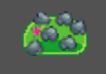
\includegraphics[width=0.4\textwidth]{slime_rock.png}
                    \caption{Slime de Roche}
                    \label{fig:mesh1}
                \end{figure}

                Cette soutenance ajoute une mise à jour majeure de notre jeu, en effet, nous avons pu implémenter notre première transformation, qui est le point central de notre jeu. Cette première transformation nous permet de changer d’apparence pour le slime afin de reconnaître visuellement notre transformation actuelle. Cette transformation est propre à chaque joueur, nous devons encore décider du fait de pouvoir se transformer. La transformation en slime de pierre permet de faire des roulades sur les murs pour les escalader, et de lancer des pierres afin de tuer les ennemis. Durant les semaines à venir, nous serons amenés à créer de nouvelles transformations.

                Pour se transformer, le joueur doit entrer en contact avec un rocher tagué avec le type caillou. Pour créer la forme de roche, on a collé des rochers sur la forme du slime de base et le faire rotationner afin de créer l’animation de roulade. Il prend alors la forme de rocher et débloque deux capacités: la roulade et le lancer de caillou. Pour la roulade, on a mis des capteurs de chaque côté (un peu comme la technique de saut du villageois au début, voir partie IA) qui lorsque le joueur est en transformation roche et en contact avec un mur lui permet de faire la roulade lui permettant de grimper le mur en appuyant sur une touche prédéfinie (flèche haut), la gravité est enlevé lors de la grimpe ainsi que le mouvement horizontal. Ensuite, il a fallu réguler des valeurs afin que le slime ne se retrouve pas coincé au bord d’un mur. Pour gérer toutes ces animations il a fallu créer de nombreux booléen dans l’animator (un pour la forme de rocher, un pour la transition en roulade et un pour son animation de blessé en forme rocher).

                Lors de notre transformation en slime rocheux, nous avons la possibilité avec la touche P de tirer un cailloux devant le slime, cela permet de tuer des ennemis à distance, cette capacité a été implémenté de manière à que les projectiles soit instanciés via photon à partir d’un LaunchOffset qui est l’endroit où spawn le projectile. Le projectile est détecté à partir d’un tag don si ce caillou touche la zone faible de l’ennemi (Weakspot) cet ennemi mourra.
                Ils bougent en ligne droite et sont détruits dès qu’ils touchent soit un ennemi soit un obstacle.

                De plus, nous avons modifié la transformation du slime rocheux. Effectivement, il n’est désormais plus possible de tirer des pierres afin d’éliminer les ennemis, cette transformation n’est désormais utile que pour le déplacement.
            \end{indt}

            \begin{indt}{\subsubsection{Slime de Feu}}
                \begin{figure}[h]
                    \centering
                    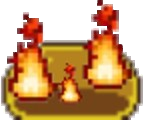
\includegraphics[width=0.4\textwidth]{SlimeDeFeu.png}
                    \caption{Slime de Feu}
                    \label{fig:mesh1}
                \end{figure}

                Afin de compenser cette perte de capacité, nous avons mis en place un slime de feu, qui à la capacité de lancer des petites flammes permettant de combattre les ennemis.

                En effet, le slime de feu sera surtout utile dans le second niveau qui contrairement au premier niveau est plus centré sur l’affrontement d’ennemis que le parcours de chemin montagneux. Ainsi, grâce à la transformation de feu, le joueur pourra attaquer ses ennemis à distance. Pour réaliser cela, nous nous sommes inspirés de ce que l’on avait fait pour le lancer de cailloux en remplaçant cela par des boules de feux.Toutefois, nous avons tout de même dû régler de nombreux bugs.

                Tout d’abord, nous avons fait en sorte de pouvoir tirer des boules de feux dans les deux sens en distinguant deux cas et en ajoutant une source pour faire apparaître les boules de feux des deux côtés du slime.

                Afin de compenser cette perte de capacité, nous avons mis en place un slime de feu, qui à la capacité de lancer des petites flammes permettant de combattre les ennemis.

                En effet, le slime de feu sera surtout utile dans le second niveau qui contrairement au premier niveau est plus centré sur l’affrontement d’ennemis que le parcours de chemin montagneux. Ainsi, grâce à la transformation de feu, le joueur pourra attaquer ses ennemis à distance. Pour réaliser cela, nous nous sommes inspirés de ce que l’on avait fait pour le lancer de cailloux en remplaçant cela par des boules de feux.Toutefois, nous avons tout de même dû régler de nombreux bugs.

                Tout d’abord, nous avons fait en sorte de pouvoir tirer des boules de feux dans les deux sens en distinguant deux cas et en ajoutant une source pour faire apparaître les boules de feux des deux côtés du slime.

                Le sprite du slime de feu présente un slime de base dans une teinte orange vif. Des flammes sont habilement incorporées au design du sprite, créant un effet visuel saisissant. Les contours du slime sont accentués par des langues de flammes qui dansent et ondulent autour de lui, évoquant la puissance et l'énergie du feu. Cette combinaison entre la forme familière du slime et les éléments du feu confère au sprite du slime de feu une apparence distinctive et captivante.

                Ensuite, il a fallu réaliser les animations liées à cette transformation tel que l’idle, le saut, … (voir photos), ainsi que les transitions entre les différentes animations (voir l’animator du slime dans la partie animation).
            \end{indt}
        \end{indt}

        \newpage

        \begin{indt}{\subsection{Intelligence Artificielle}}
            \begin{indt}{\subsubsection{Sanglier}}
                \begin{figure}[h]
                    \centering
                    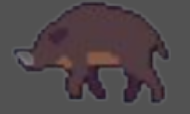
\includegraphics[width=0.5\textwidth]{sanglier.png}
                    \caption{Le sanglier}
                    \label{fig:mesh1}
                \end{figure}

                Nous avons décidé d’implémenter l’IA via les différents ennemis. En effet, chaque ennemi a un comportement différent selon ses capacités et/ou ce que fait le joueur. Pour l’instant, un seul ennemi a été implémenté: le sanglier. Ce dernier se déplace entre deux points définis au préalable. En effet, à chaque instant le programme vérifie la position du sanglier par rapport à un des deux points qui est ciblé et tant qu’il n’a pas atteint ce point  il avance vers ce point avec une vitesse prédéfinie. Lorsqu’il atteint le point visé, il prend le second point pour cible et commence à avancer vers lui.

                Par rapport au joueur, il ne change de comportement que lorsque ce dernier lui saute dessus, c'est-à-dire lorsque la zone de contact du slime et une zone au-dessus du sanglier entrent en contact. Le sanglier va alors lancer son animation de mort et s’autodétruire 0,5 seconde après le contact. De plus, le joueur sera propulsé dans les airs grâce à un attribut de PhysicMaterial 2D avec une propriété de rebondissement. Cette technique de patrouille entre deux points  peut aussi être adaptée afin de faire en sorte que l’ennemi poursuit le joueur tout simplement en mettant le point visé sur le joueur ce qui pourra être utile pour de prochains ennemis.

                Une autre technique qui a été envisagée pour faire patrouiller l’ennemi est de le faire avancer jusqu'à ce qu’il se cogne dans un objet différent du joueur (mur, objet solide, …), le faisant repartir dans l’autre sens. L’inconvénient avec cette technique c’est que si il y a une zone de vide l’ennemi ne va pas s’arrêter et tomber dans le vide, contrairement à la patrouille actuelle où l’ennemi ne dépasse jamais le point cible.

                Finalement, nous avons remplacé les deux points par un zone appelée Monster area. Le principe reste le même, le sanglier patrouille dans la zone délimitée. Cela permet d’utiliser moins d’objets dans la scène et permet une synchronisation en multijoueur plus simple.

                Le sanglier possède donc deux animations: son animation où il court (toujours active tant qu’il n’est pas attaqué) et son animation de mort qui s’active lorsque le joueur lui saute dessus.

                Au niveau des effets sonores, il possède un son de mort qui se joue brièvement après son élimination.

                Pour le deuxième soutenance, nous avons développé deux nouvelles IA ennemis, la première suit le joueur sur une certaine distance, afin d’ajouter de la difficulté au jeu, la seconde quant à elle, permet à un archer de tirer des flèches en direction du joueur, ce qui rend le jeu définitivement plus dur, nous permettant aussi une création de niveau plus souple, nous permettant de gérer les attributs des IA afin d’accentuer ou de diminuer la difficulté. Des pièges ont aussi été ajoutés, mais ils sont une forme d’IA encore plus basique que les autres.
            \end{indt}

            \begin{indt}{\subsubsection{Le Villageois}}
                \begin{figure}[h]
                    \centering
                    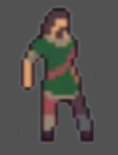
\includegraphics[width=0.3\textwidth]{villageois.png}
                    \caption{Le villageois}
                    \label{fig:mesh1}
                \end{figure}

                Nous voulions créer un ennemi hostile au joueur qui le suit dès qu’il se rapproche un peu trop de lui. Tout d’abord on utilisait des vecteurs afin de rediriger le villageois vers le joueur. Cependant, cela faisait que le villageois traversait tous les murs afin d’atteindre l' utilisateur. Nous avons donc utilisé un rigidbody auquel on ajoute des forces en direction du joueur ce qui a permis de résoudre ce problème et d’avoir un mouvement plus naturel.

                Ensuite, on voulait faire en sorte que le villageois saute lorsqu'il se cogne contre un mur afin de poursuivre le joueur jusqu’au bout. On a donc ajouté des capteurs de chaque côté du villageois qui lorsqu’ils entrent dans un mur font sauter le villageois. Le problème était que les villageois étaient trop forts. En effet, il était presque impossible de lui échapper à moins de le feinter. Nous avons donc décidé de garder cette technique de saut pour plus tard. On a donc enlevé cette partie de code et appliqué un matériel de type Trampoline au joueur afin d’avoir un villageois un peu plus naturel (contrairement à avant où il volait presque). On lui a aussi ajouté ses animations de mort, de déplacements et d’attaque.

                Pour l’éliminer, on a d’abord implémenté la même technique que pour le sanglier (lui sauter sur la tête). Ensuite, avec le développement de la transformation du slime, on peut maintenant éliminer le villageois en lui laissant les boules de feux de la transformation en feu du slime.
                Au niveau sonore, il possède un son de mort afin de bien signaler à l’utilisateur que le villageois a été éliminé.
            \end{indt}

            \begin{indt}{\subsubsection{L’archer}}
                \begin{figure}[h]
                    \centering
                    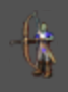
\includegraphics[width=0.3\textwidth]{archer.png}
                    \caption{L'archer}
                    \label{fig:mesh1}
                \end{figure}

                Pour l’archer, nous cherchions un ennemi qui puisse imposer une nouvelle difficultée au joueur. Après avoir trouvé les sprites d’un archer avec ses flèches, nous avons commencé par créer l’animation de tir de l’archer. Ensuite on lui a associé une source au niveau du bout de l’arc qui sera l’endroit où sortiront les flèches. On lui associé un timer dans le script afin de tirer les flèches toutes les 2 secondes et éviter que ce dernier spamme les flèches non-stop et sans être coordonné avec l’animation de tir. On a ensuite ajouté un rigidbody aux flèches pour pouvoir leur ajouter une force vers le joueur. On leur a donné un tag ennemi afin que lorsque les flèches arrivent sur le joueur, le joueur prenne des dégâts.  Ensuite on a dû régler un problème qui faisait que les flèches ne disparaissaient pas après avoir cogné un objet. On a donc activer le Trigger sur le BoxCollider des flèches ce qui a permis de faire traverser les flèches à travers tous les objets sauf le joueur.

                Enfin on a implémenté la même méthode d’élimination d’ennemis que le sanglier (sauter sur la tête) ainsi que la technique de lancer de boules de feu de la transformation en slime de feu.

                Au niveau du multijoueur, on a dû réimplémenter l'instanciation des flèches tout comme on a fait avec les différents ennemis car les flèches n’apparaissaient pas en multijoueur.

                Il manquait juste pour l’archer une animation de mort et le fait qu’il se retourne vers le joueur afin que les flèches apparaissent du bon côté. Nous avons donc régler ces problèmes en créant une animation qui fait varier la couleur de l’archer progressivement en rouge pour ensuite le faire disparaître. Pour qu’il se retourne nous avons fait en sorte de retourner le sprite de l’archer en utilisant le booléen flip.x. Selon la position du joueur, ce booléen passe à true et le sprite de l’archer se retourne.

                Comme les autres ennemis, au niveau sonore, l’archer à un effet sonore lorsqu'il est éliminé par l’utilisateur.
            \end{indt}

            \begin{indt}{\subsubsection{Piège à ours}}
                \begin{figure}[h]
                    \centering
                    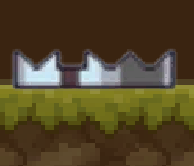
\includegraphics[width=0.5\textwidth]{piege_a_ours.png}
                    \caption{Le piège à ours}
                    \label{fig:mesh1}
                \end{figure}

                On a ensuite voulu développer des pièges afin de complexifier les zones de parcours des niveaux. Pour le piège à ours, on lui a créé une zone de détection qui s’active lorsqu’un objet de type Player rentre dans la zone.  Au moment où le joueur rentre dans la zone l’animation du piège qui se referme se lance à l’aide d’un booléen dans l’animateur puis reste refermer. Afin que le joueur ne reprenne plus dégâts lorsque le piège est fermé, la zone de détection du joueur est détruite.

                Nous avons aussi eu l’idée de permettre au joueur d’activer ces pièges à distance. En effet, en utilisant la même technique qu’avant nous avons fait en sorte d'activer le piège à ours lorsqu’un projectile du joueur passe dessus. Cela permet de faciliter le parcours du joueur de façon astucieuse et risque d’être très utile à l’avenir…

                Ces pièges sont dissimulés dans les niveaux afin de surprendre certains joueurs qui feraient du tout droit non stop. Nous avons envisagé de pouvoir faire en sorte que cela bloque le joueur pendant quelques secondes mais nous avons pensé que cela nuirait à la fluidité du parcours du niveau.
            \end{indt}

            \begin{indt}{\subsubsection{Piques}}
                \begin{figure}[h]
                    \centering
                    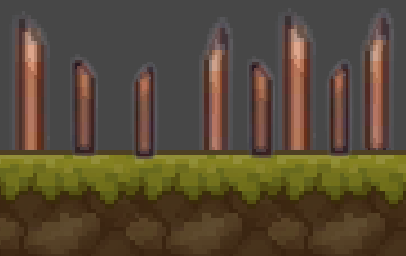
\includegraphics[width=0.5\textwidth]{pique.png}
                    \caption{Les piques}
                    \label{fig:mesh1}
                \end{figure}

                Les piques sont un piège assez basique avec un box collider et un tag Ennemi qui permet de faire des dégâts au joueur lorsque ce dernier tombe dans le ravin remplis de piques. Au début le joueur mourrait directement car il prenait les dégâts de plusieurs piques à la fois. Cependant, grâce à la mise en place d’un cooldown sur les dégâts prit par le joueur, le joueur ne meurt plus instantanément.

                Ces piques permettent d’obliger le joueur à utiliser ces compétences de roche et de parcours dans le niveau un mettant vraiment en valeur l’utilité de l’escalade en mode roche.

                Pour cette troisième soutenance le but était d’implémenter le boss de notre jeu ainsi que d’apporter des améliorations aux autres ennemis. On a aussi eu l’idée de l'implémentation d’une mécanique de soin comme vous le verrez ci-dessous.
            \end{indt}

            \newpage

            \begin{indt}{\subsubsection{Pomme}}
                \begin{figure}[h]
                    \centering
                    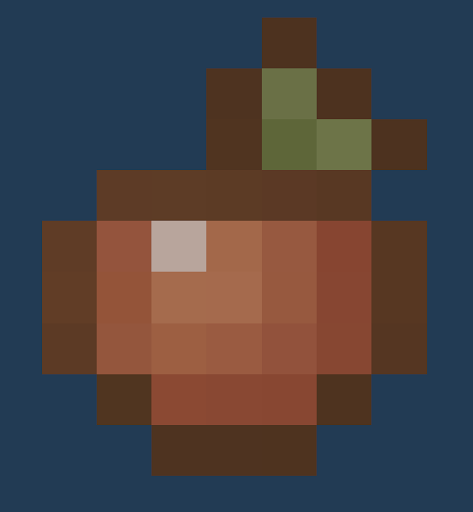
\includegraphics[width=0.3\textwidth]{Pomme.png}
                    \caption{La pomme}
                    \label{fig:mesh1}
                \end{figure}

                La pomme est le seul objet capable de redonner une vie au joueur. Nous voulions introduire cette mécanique de soin au jeu afin de permettre au joueur de pouvoir récupérer des vies qu’il aurait bêtement perdues et qui seront de grande aide pour affronter les ennemis et le boss. Tout d’abord, pour que le joueur détecte la pomme lorsqu’il la touche nous avons attribué à la pomme un box collider avec un tag de type “heal”.

                Ensuite on a fait la distinction de trois cas (comme pour les dégâts). Soit le joueur a déjà toutes ses trois vies il ne se passe rien dans ce cas, soit le joueur a deux vies, on lui réactive alors le troisième coeur et lui met sa vie à trois, soit il n’a qu’une vie et alors on lui met sa vie à deux et on réactive le deuxième coeur. Un effet sonore a été ajouté au slime afin que le joueur puisse savoir s' il a pris la pomme sachant que la pomme disparaît au contact du joueur.

                Comme tous les autres ennemis, la pomme est instanciée par Photon et possède un Photon view afin d’éviter les problèmes de synchronisation en multijoueur.
            \end{indt}

            \begin{indt}{\subsubsection{Bûcheron}}
                \begin{figure}[h]
                    \centering
                    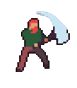
\includegraphics[width=0.5\textwidth]{Bucheron.png}
                    \caption{Le bûcheron}
                    \label{fig:mesh1}
                \end{figure}

                Le bûcheron est le boss du village du second niveau. Nous voulions absolument avoir un boss dans notre jeu afin d’apporter plus de challenges aux joueurs. En effet, le bûcheron n’est pas un simple ennemi qui meurt en un coup ou une boule de feu.

                Ce dernier possède une barre de vie avec un certain nombre de points de vie. Cette barre de vie a été réalisée grâce à un Slider (un objet de type Canvas) qui permet de plus ou moins remplir une jauge à l’aide d’une valeur comprise entre zéro et un. Afin que le remplissage du Slider corresponde bien aux nombres de points de vie du boss à tout moment, nous mettons à jour la valeur du Slider en faisant le calcul suivant : le nombre de points de vie actuel divisé par le nombre de points de vie maximale. Il a fallu faire de nombreux ajustements sur la quantité de points de vie afin que le boss ne soit pas trop simple mais pas trop long et répétitif non plus.  Pour l'éliminer, le joueur doit lui mettre assez de dégâts pour ramener sa vie à zéro, cependant ceci est plus facile à dire qu'à faire.

                Le bûcheron est l’IA la plus développée du jeu, il regroupe des mécaniques que d’autres ennemis avaient tout en apportant de nouvelles. Il a deux phases différentes, la transition entre les deux se faisant lorsqu’il est à la moitié de sa barre de vie.

                Pour la première phase, le bûcheron va se contenter de poursuivre le joueur en essayant de lui asséner des coups. Un peu comme pour le villageois, à partir du moment où le joueur rentre dans la zone de détection du bûcheron, ce dernier va se tourner vers lui et lui courir dessus. Pour cela, un objet de type rigidbody lui est attaché et auquel on rajoute des forces en direction du joueur. Mais ce n’est pas tout. Le joueur, voyant le bûcheron s’approcher de lui à pleine vitesse, pourrait penser qu’il suffit juste de lui sauter par-dessus comme pour le villageois mais c’est là qu’il se trompe. Si le bûcheron est à une certaine intervalle de distances du joueur (on ne va pas donner de chiffres vous le devinerez vous même en jouant), alors il va parfois lancer un saut plus ou moins grand (en ajoutant une force verticale au rigidbody). En effet, plus le joueur reste à la même distance du bûcheron, plus le saut du bûcheron va être grand. Cela permet de surprendre certains joueurs trop attentistes pensant pouvoir simplement spammer depuis le même endroit.

                La deuxième phase est marquée par une animation du bûcheron où l’on voit ce dernier se mettre en colère. Pour la seconde phase, toutes les techniques précédentes sont conservées mais on y ajoute le tir d’arc du bûcheron. Ce tir s'enclenche deux fois: une première fois lorsque le bûcheron arrive à la moitié de ses points de vie et une deuxième fois lorsqu’il ne reste plus qu’un quart de ses points de vie. Le bûcheron va s’élever d’un coup dans les airs et enclenché son animation de tir de l’arc. Ensuite une flèche spéciale (voir photo ci-dessous) va apparaître (via Photon pour la synchronisation en multijoueur bien évidemment), est va se diriger vers l'emplacement du joueur lors du tir de la flèche. Comme les flèches de l’archer, elle traverse tous les objets et disparaît au bout de quelques secondes. Les différences majeures avec la flèche normale de l’archer est sa taille, sa vitesse, mais surtout le fait qu’elle est une animation afin de rendre le projectile plus fluide et dangereux. Cette flèche est donc bien plus dure à esquiver que les flèches normales et risquent de faire perdre de nombreuses vies aux joueurs imprudents.

                \begin{figure}[h]
                    \centering
                    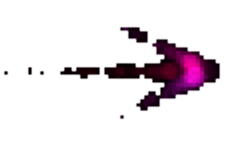
\includegraphics[width=0.5\textwidth]{Arrow.png}
                    \caption{Le projectile}
                    \label{fig:mesh1}
                \end{figure}

                A tout cela s’ajoute tout un système d’animation que ce soit pour la course du bûcheron, son attaque, son animation de dégâts, de mort, de tirs et d’énervement. Tout cela étant relié par de nombreuses transitions.

                Enfin, au niveau sonore il y a bien évidemment des effets sonores signalant que le bûcheron a été blessé (en plus de l’animation), son son de mort et de début de deuxième phase.
            \end{indt}
        \end{indt}

        \newpage

        \begin{indt}{\subsection{Animations}}
            Pour les animations, nous avions déjà implémenté les animations de base (inactif, saut, dégât, roulade en transformation roche). Nous avons donc décidé de rajouter certaines animations que nous trouvions indispensables pour la fluidité du jeu, notamment pour les dégâts ou les sauts. Pour certaines animations, il était important d’instaurer un ordre de priorités. Par exemple, nous devrions pouvoir utiliser l’animation de roulade depuis n’importe quelle animation du slime roche.  Pour ce faire, nous avons créé un niveau dans l’animator (composant de Unity pour gérer les transitions entre animations) du joueur.

            Tout cela c’est encore plus complexifié avec l’ajout de la transformation de feu. Grâce aux paramètres (booléen, trigger, …) nous avons pu coordonnées toutes ces animations avec les nombreuses transitions que vous voyez.

            Le plus dur a été de trouver les transitions entre les animations qu’ils manquaient car le seul moyen de le savoir était de tester des cas très précis. De plus, plus on ajoute d’animations, plus le nombre de cas à gérer augmente.

            \begin{figure}[h]
                \centering
                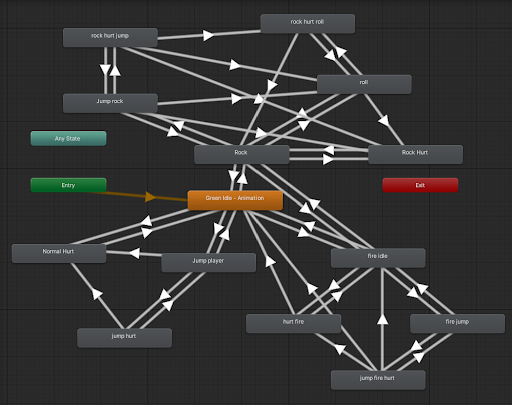
\includegraphics[width=0.5\textwidth]{Annim1.png}
                \caption{Annimator du Slime}
                \label{fig:mesh1}
            \end{figure}

            De même l’animation du boss final est commandée par un animator. Les transitions vers l’animation Angry permettent d’activer visuellement la seconde phase du boss dès que le moment est venu. Toutes ces transitions sont nécessaire afin de d’assurer que le boss fasse les animations en accord avec ces attaques et mouvements.

            \begin{figure}[h]
                \centering
                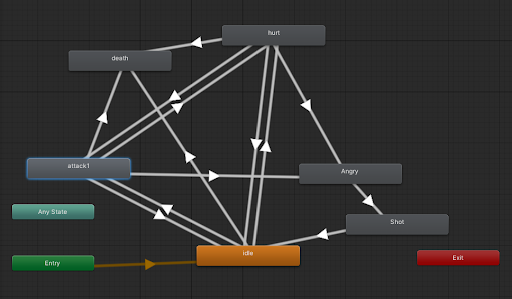
\includegraphics[width=0.5\textwidth]{Annim2.png}
                \caption{Annimator du Boss}
                \label{fig:mesh1}
            \end{figure}

            Bien évidemment, nous utilisons aussi ce système de transitions pour tous les objets animés. Que ce soit le sanglier, l’archer, le villageois, le piège à ours, le trésor de fin de niveau, et même les flèches spéciales du boss (animation de idle). Pour la plupart de ces objets, ils n’ont pas plus de trois animations différentes : une animation de idle, une animation de mort et parfois une animation d'attaques.
        \end{indt}

        \begin{indt}{\subsection{Les Différents Niveaux}}
            Note jeu “A Slime’s journey”, se joue en plusieurs niveaux avec une progression adaptée que ce soit au niveau de la difficulté mais aussi du voyage qu'entreprend le slime. Ces niveaux sont l’image du scénario que vous avez pu lire ci-dessus.

            La transition entre chaque niveau se fait à l’aide de téléporteurs. En effet, lorsque le joueur arrive à la fin du niveau, il y a un objet (panneau, porte, …) avec une certaine étiquette qui s’active lorsque le joueur rentre en contact avec. Cela va téléporter le joueur au prochain niveau.

            Au départ, nous avions prévu de faire chaque niveau dans une scène Unity différente mais cela posait des problèmes importants de synchronisation en multijoueur. Nous avons donc fait les trois niveaux dans la même scène en faisant les transition avec les téléporteurs qui changent les coordonnées du joueur.

            \begin{indt}{\subsubsection{Premier niveau}}
                \begin{figure}[h]
                    \centering
                    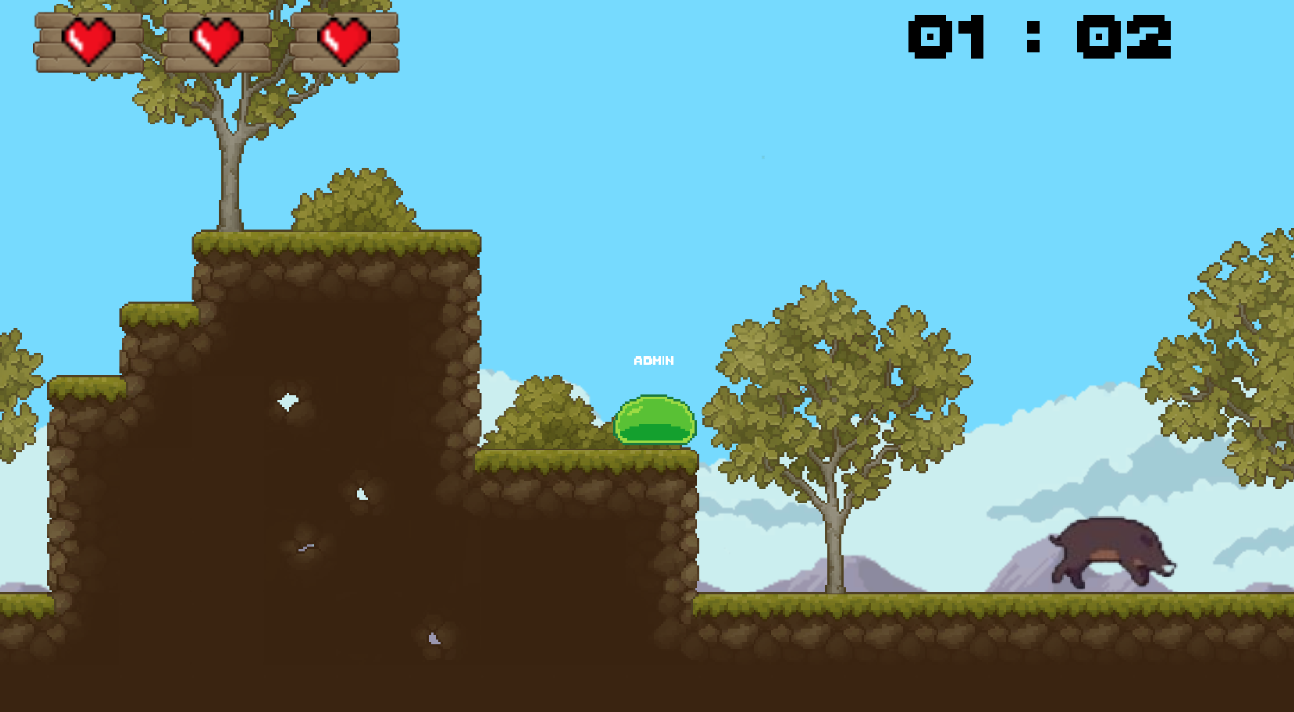
\includegraphics[width=0.5\textwidth]{niv1.png}
                    \caption{Premier niveau}
                    \label{fig:mesh1}
                \end{figure}

                Le premier niveau est un niveau d’initiation au jeu. La difficulté du niveau n’est pas très élevée et permet aux joueurs de découvrir le jeu et ses mécaniques notamment celle de transformation.

                Du point de vue de l'histoire de “A Slime’s journey”, ce premier niveau marque le début de l’aventure de notre chère slime qui parcourt le royaume afin d’un jour affronter le roi. Mais avant cela, il doit ce sortir de cette plaine remplie d'embûches.

                Le game design de ce jeu a énormément changé entre les différentes soutenances mais aussi au niveau graphique. Finalement, la dernière version de ce niveau permet véritablement au joueur de bien débuter tout en mettant en valeur l’utilité de la transformation roche.

                En effet, dans ce niveau, de nombreux dénivelés de terrain et pièges (tels que les piques et les pièges ours présentés ci-dessus) inscrit vraiment notre jeu dans le style de jeu de plateformes de part la nécessité de réaliser des sauts et des parcours en mode roulade de roche plus ou moins compliqué.

                \begin{figure}[h]
                    \centering
                    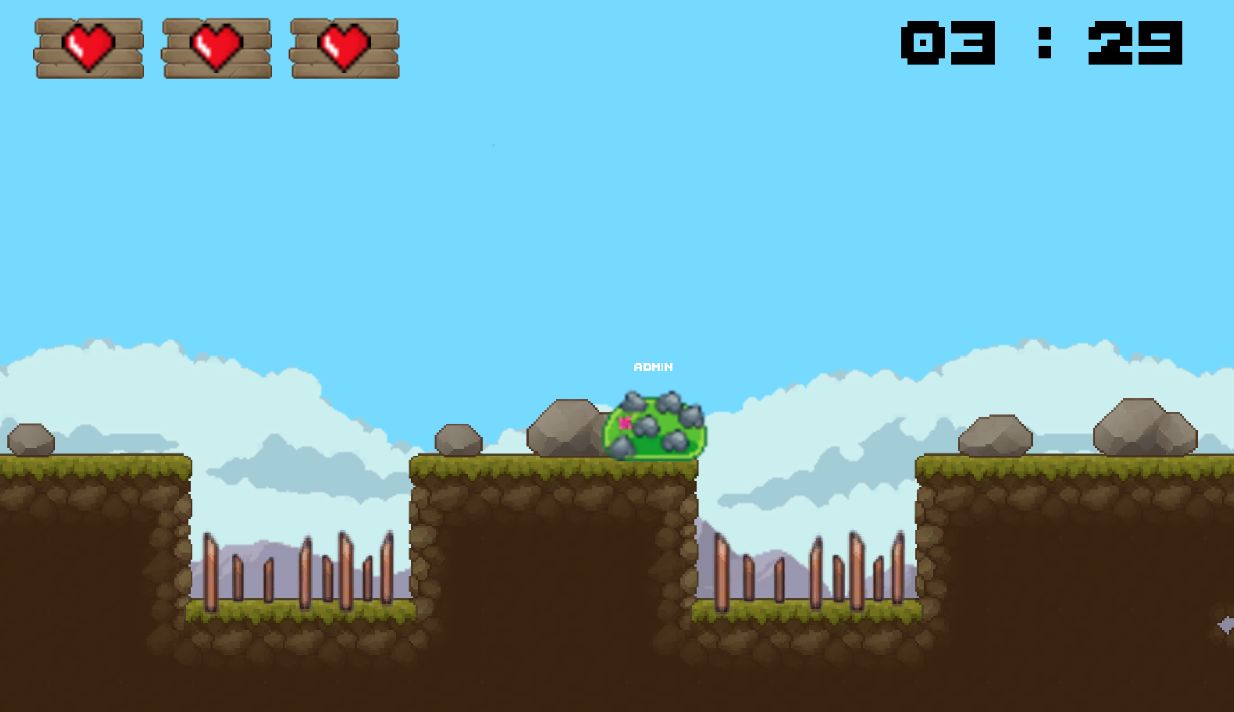
\includegraphics[width=0.5\textwidth]{niv1_rck.png}
                    \caption{Fin du premier niveau}
                    \label{fig:mesh1}
                \end{figure}

                C’est aussi l’occasion pour le joueur de faire face à son premier ennemi : le sanglier. Ce sanglier, bien que pas très coriace, permet au joueur d’apprendre à sauter sur les ennemis pour les éliminer.

                Enfin, après avoir dépassé tous les obstacles, le joueur va rentrer dans une caverne qui va le mener au second niveau.
            \end{indt}

            \begin{indt}{\subsubsection{Niveau deux}}
                Le second niveau lui a été développé avant la deuxième soutenance mais a subi une refonte totale au niveau graphique permettant ainsi d’avoir un niveau plus plaisant pour le joueur visuellement. Le game design de ce niveau a aussi été quelque peu modifié afin d’avoir une progression plus fluide.

                \begin{figure}[h]
                    \centering
                    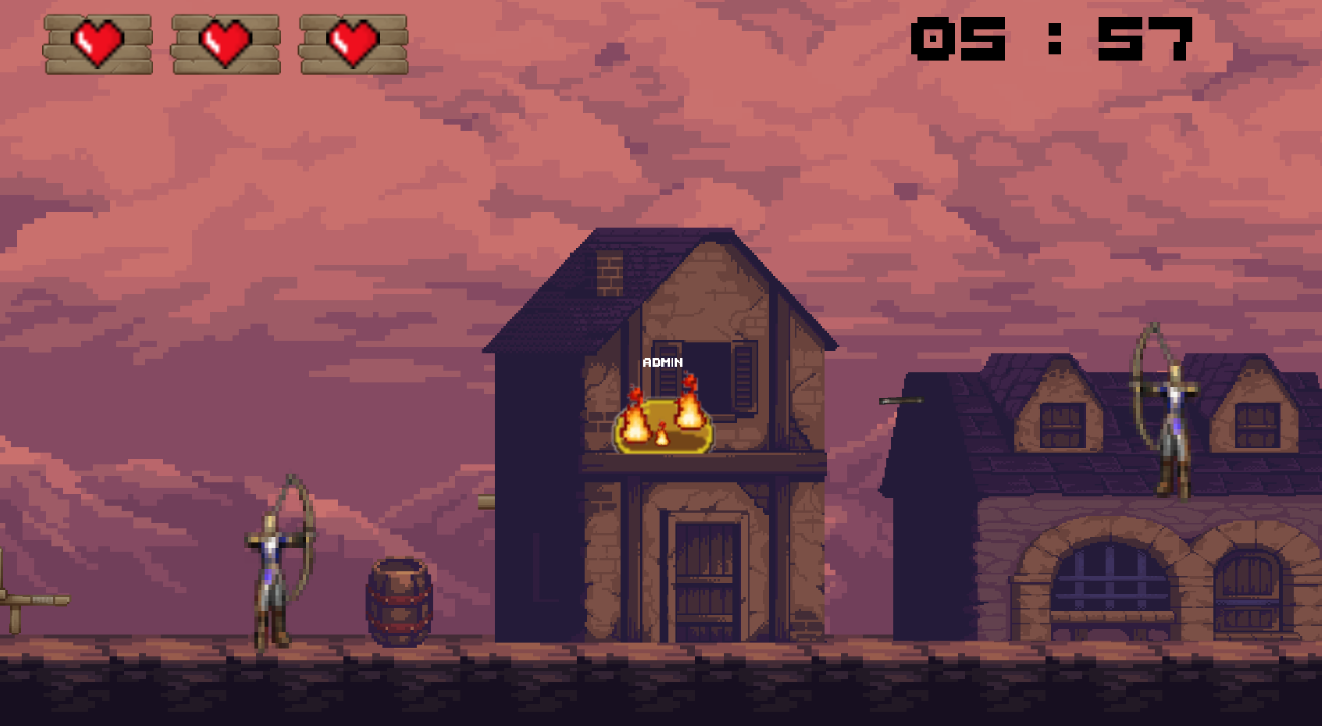
\includegraphics[width=0.5\textwidth]{niv2_fire.png}
                    \caption{Deuxième niveau}
                    \label{fig:mesh1}
                \end{figure}

                Dans ce niveau l’accent a été mis sur le combat d’ennemis permettant aux joueurs de tester leurs compétences face à un premier véritable challenge.

                Ce niveau prend la suite du niveau un. En effet, après être sorti de la caverne, le slime arrive dans un village. Cependant, ces habitants voyant un monstre arrivé prennent les armes pour l’affronter. Il ne sera pas chose facile au slime de traverser ce village rempli d’ennemis mais c’est là que la transformation de feu du slime rentre en jeu.

                Le slime de feu ayant la capacité de tirer des boules de feu peut éliminer ces adversaires avec. Toutefois, ces derniers ne se laisseront pas faire. Dans ce niveau vous retrouvez le villageois et l’archer qui contrairement au sanglier vont directement essayer d’attaquer le slime (voir partie IA ci-dessus). Le joueur pourra se servir de l’environnement pour se mettre à couvert des tirs ennemis (caisse, tonneau, …) ou au contraire pour sauter sur les toits afin d’attaquer ses adversaires en hauteur.

                Heureusement, il y a aussi dans ce niveau des pommes qui permettent au slime de regagner une vie s’il a été blessé lors des combats. De plus, nous avons spécialement mit deux pommes à la fin du niveau afin que le joueur passe au niveau suivant (qui sera un peu plus corsée) avec toutes ses vies.

                Après avoir traversé le village, le joueur arrive à la porte d’un grand donjon qui va le mener au dernier niveau.

                \begin{figure}[h]
                    \centering
                    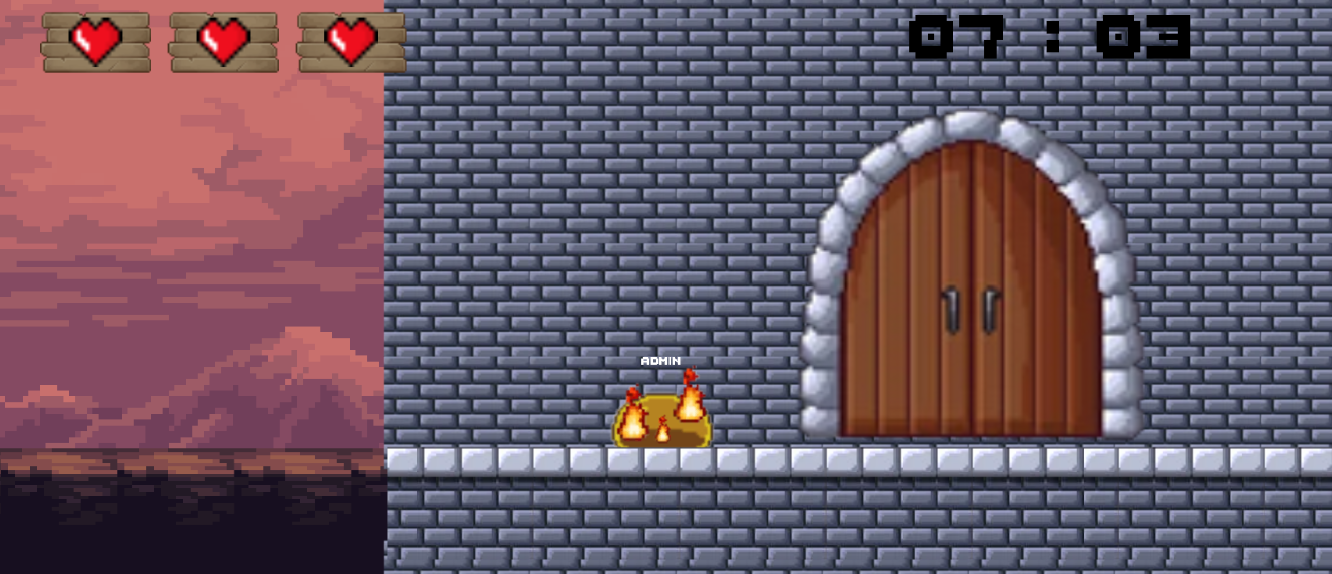
\includegraphics[width=0.6\textwidth]{entree_chateau.png}
                    \caption{Fin du deuxième niveau}
                    \label{fig:mesh1}
                \end{figure}
            \end{indt}

            \newpage

            \begin{indt}{\subsubsection{Niveau trois}}
                Le troisième niveau est un combat de boss face au chef du village: le bûcheron. Le slime se retrouve dans une pièce froide, fermée, truffée de pièges, face au chef du village qu’il vient de traverser.

                \begin{figure}[h]
                    \centering
                    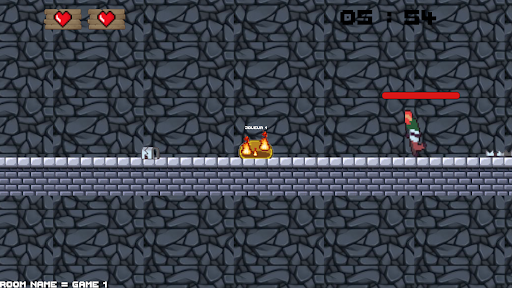
\includegraphics[width=0.5\textwidth]{Boss1.png}
                    \caption{Combat avec le Boss}
                    \label{fig:mesh1}
                \end{figure}

                Ce niveau de combat de boss permet au joueur d’affronter un ennemi de taille, bien plus complexe que les précédents. Comme dit précédemment le boss à plusieurs phases et ne meurt pas en un ou deux coups. De plus, le bûcheron voyant le slime arrivé a laissé de nombreux pièges à ours dans la salle ce qui rend le combat encore plus complexe. C’est donc une rude épreuve pour le joueur, mais il peut compter sur toutes les compétences qu’il a acquises en complétant le niveau deux.

                Après avoir vaincu le bûcheron, un coffre va apparaître que le joueur va pouvoir prendre et qui va le transporter vers l’écran de fin de jeu.

                \begin{figure}[h]
                    \centering
                    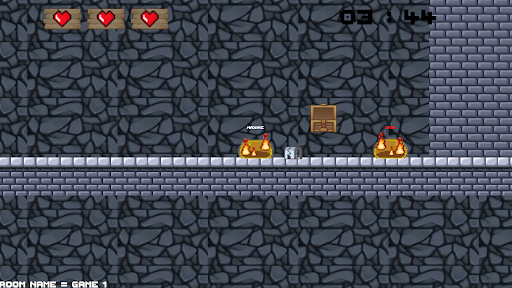
\includegraphics[width=0.5\textwidth]{Boss2.png}
                    \caption{Récompence du Boss}
                    \label{fig:mesh1}
                \end{figure}
            \end{indt}
        \end{indt}

        \newpage

        \begin{indt}{\subsection{Musique et Son}}
            Nous cherchions des musiques qui entrent dans l'univers de notre jeu. Ainsi, après de nombreuses recherches et tests sur audacity nous avons trouvé un asset de musiques qui correspondait parfaitement à l'ambiance que l'on voulait donner au jeu. En effet, en plus de coller à l'ambiance médiévale, ces musiques correspondent bien au premier niveau où l'atmosphère est plus posée et joyeuse permettant ainsi aux joueurs de mieux s'intégrer dans l'univers de “A Slime's Journey”.

            Nous avons donc utilisé quelques musiques de l'asset Fantasy RPG adventure disponible sur le Unity Asset Store. Nous utilisons deux musiques différentes : une pour le menu et une pour le premier niveau. Pour chaque scène nous avons ajouté un élément vide avec un attribut Audio Source qui permet de jouer la musique. Les effets sonores n'ont quant à eux pas encore été implémentés mais le principe reste le même qu'avec les musiques en fond, il suffit juste de les activés aux moments opportuns.
        \end{indt}

        \begin{indt}{\subsection{Les Menus}}
            \begin{indt}{\subsubsection{Menu Principal}}
                Le menu principal est la première chose que l’utilisateur voit en lançant le jeu. Nous avons donc mit beaucoup d’attention à créer une atmosphère accueillante et apaisante afin de bien introduire le jeu au joueur que ce soit au niveau visuel mais aussi sonore avec une musique très douce et relaxante.

                \begin{figure}[h]
                    \centering
                    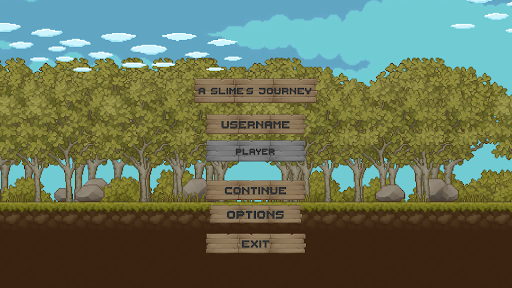
\includegraphics[width=0.5\textwidth]{Menu1.png}
                    \caption{Menu principal}
                    \label{fig:mesh1}
                \end{figure}

                Le décor du menu principal a été réalisé en utilisant les mêmes décors que pour le niveau un permettant ainsi de faire un lien logique entre le début du jeu et le menu. Afin de bien coller à l’esprit du jeu, les boutons permettant et le style d'écriture ont été choisis pour se fondre dans le décor naturellement.

                D’ailleurs, le décor est généré aléatoirement à chaque fois que le joueur va sur le menu principal. Afin d’obtenir ce résultat, les objets permettant à notre décors d’exister tel que les arbres et les rochers sont instanciées à une position aléatoire sur le sol dans l’écran

                De plus, ce décor n’est pas fixe, les nuages dans le ciel bouge doucement permettant de rendre l’environnement vivant.

                C’est depuis ce menu principal que le joueur va rentrer son pseudo ainsi que le nom de la partie qu’il souhaite créer pour ensuite se lancer dans le jeu. Le joueur peut aussi quitter et fermer le jeu en utilisant le bouton “Exit”.

                Enfin, le menu principal permet aussi d'amener à notre second menu, le menu options.
            \end{indt}

            \begin{indt}{\subsubsection{Menu Options}}
                Le menu option est là où le joueur va commencer à pouvoir personnaliser son expérience de jeu. Dans ce menu là, il va pouvoir ajuster la résolution de son jeu ainsi que le volume sonore du jeu.

                \begin{figure}[h]
                    \centering
                    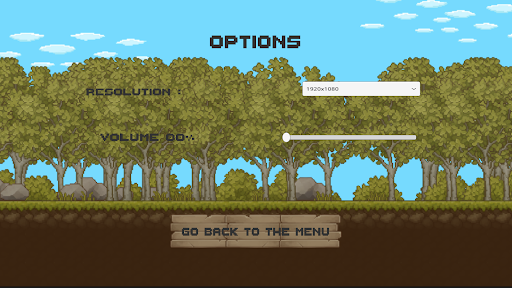
\includegraphics[width=0.5\textwidth]{Menu2.png}
                    \caption{Options du menu principal}
                    \label{fig:mesh1}
                \end{figure}

                Le joueur a aussi la possibilité de revenir au menu principal en utilisant le bouton en bas de l’écran. La police d'écriture et le style de bouton sont les mêmes que dans le menu principal tout comme le décor en fond d’écran.
            \end{indt}

            \begin{indt}{\subsubsection{Menu de Personnalisation de Touches}}
                Nous souhaitions ,depuis le début du projet, pouvoir donner aux joueurs la possibilité de personnaliser leur aventure afin d'avoir une meilleure expérience. Or, nous savons que chaque joueur à ses habitudes propres en termes de commandes de jeux, c’est pour cela que nous avons décidé de créer un menu de personnalisation de touches.

                Ce menu est accessible en pleine partie et permet au joueur d’apprendre les touches s’il ne les connaissait pas et de les modifier à sa guise tout en gardant un œil sur le jeu.

                \begin{figure}[h]
                    \centering
                    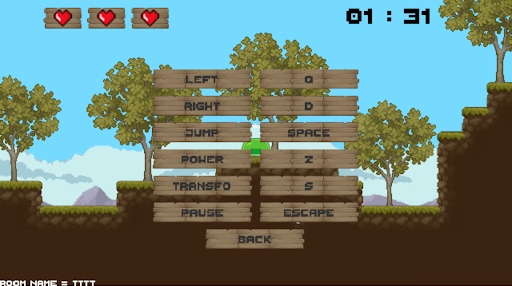
\includegraphics[width=0.5\textwidth]{Menu3.png}
                    \caption{Menu de personnalisation des touches}
                    \label{fig:mesh1}
                \end{figure}

                Afin de permettre une personnalisation des touches, nous avons mis en place un objet scriptable, permettant d'associer certaines touches à certaines actions par la suite.
            \end{indt}

            \begin{indt}{\subsubsection{Menu de Fin de Jeu}}
                Après avoir vaincu le boss du village, le joueur va prendre le coffre et va être transporté vers le menu de fin de jeu.

                Dans ce menu, on va y retrouver un texte qui s’affiche félicitant le joueur qui à terminé le jeu et va lui donner le temps qu’il a mit à faire tous les niveaux.. Tout cela est bien évidemment accompagné d’une musique pour célébrer la victoire du joueur.

                Ensuite, le joueur va pouvoir retourner au menu principal à l’aide d’un bouton dans le menu. De là il va pouvoir soit retenter sa chance pour essayer de faire un meilleur temps soit fermer le jeu s’il le souhaite.
            \end{indt}
        \end{indt}

        \begin{indt}{\subsection{Communication}}
            Notre objectif était d'établir une présence en ligne solide en utilisant les plateformes sociales telles qu'Instagram et Discord pour atteindre notre public cible et créer une communauté engagée.

            Nous avons lancé un compte Instagram dédié (arcln$\_$prod) pour partager des visuels attrayants, des captures d'écran de gameplay et des illustrations inédites. Notre objectif était de susciter l'intérêt et l'enthousiasme parmi les abonnés grâce à du contenu régulier et engageant. Des légendes pertinentes et des hashtags ont été utilisés pour maximiser la portée des publications et encourager la participation des utilisateurs. Nous avons également organisé des concours et des cadeaux pour récompenser notre fidèle communauté et stimuler la viralité des publications.

            Parallèlement, nous avons créé un serveur Discord pour rassembler les joueurs et favoriser les échanges. Le serveur Discord comprend différents canaux dédiés aux discussions sur le jeu, aux astuces, aux questions et aux retours.

            Nos efforts de communication publique ont connu un succès encourageant, avec une croissance de notre base d'abonnés sur Instagram et une communauté active sur Discord. Nous continuerons à créer du contenu attrayant et régulier sur Instagram, en interagissant avec nos abonnés pour maintenir un dialogue ouvert. Nous organiserons également des événements engageants sur Discord pour renforcer la cohésion de la communauté et favoriser l'échange entre les joueurs et l'équipe de développement.

            Puisque la communication publique joue un rôle crucial dans la promotion et l'engagement de "A Slime's Journey". Nous sommes déterminés à poursuivre nos efforts pour créer une expérience inoubliable pour les joueurs et développer une communauté passionnée autour du jeu.

            \begin{figure}[h]
                \centering
                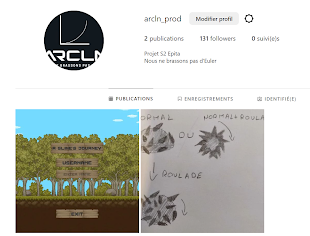
\includegraphics[width=0.5\textwidth]{Insta.png}
                \caption{Le compte Instagram du groupe}
                \label{fig:mesh1}
            \end{figure}
        \end{indt}

        \newpage

        \begin{indt}{\subsection{Jaquette}}
            Pour la jaquette contenant le jeu nous avons gardé le même décor que nos différents menu tout en s’inspirant de jaquette d'autres jeux. En effet, pour la forme de la jaquette au recto nous nous sommes inspirés de celle du premier super mario bros sur NES. On peut y trouver le slime ainsi que le bûcheron et le nom de notre jeu dans son style caractéristique.

            \begin{figure}[h]
                \centering
                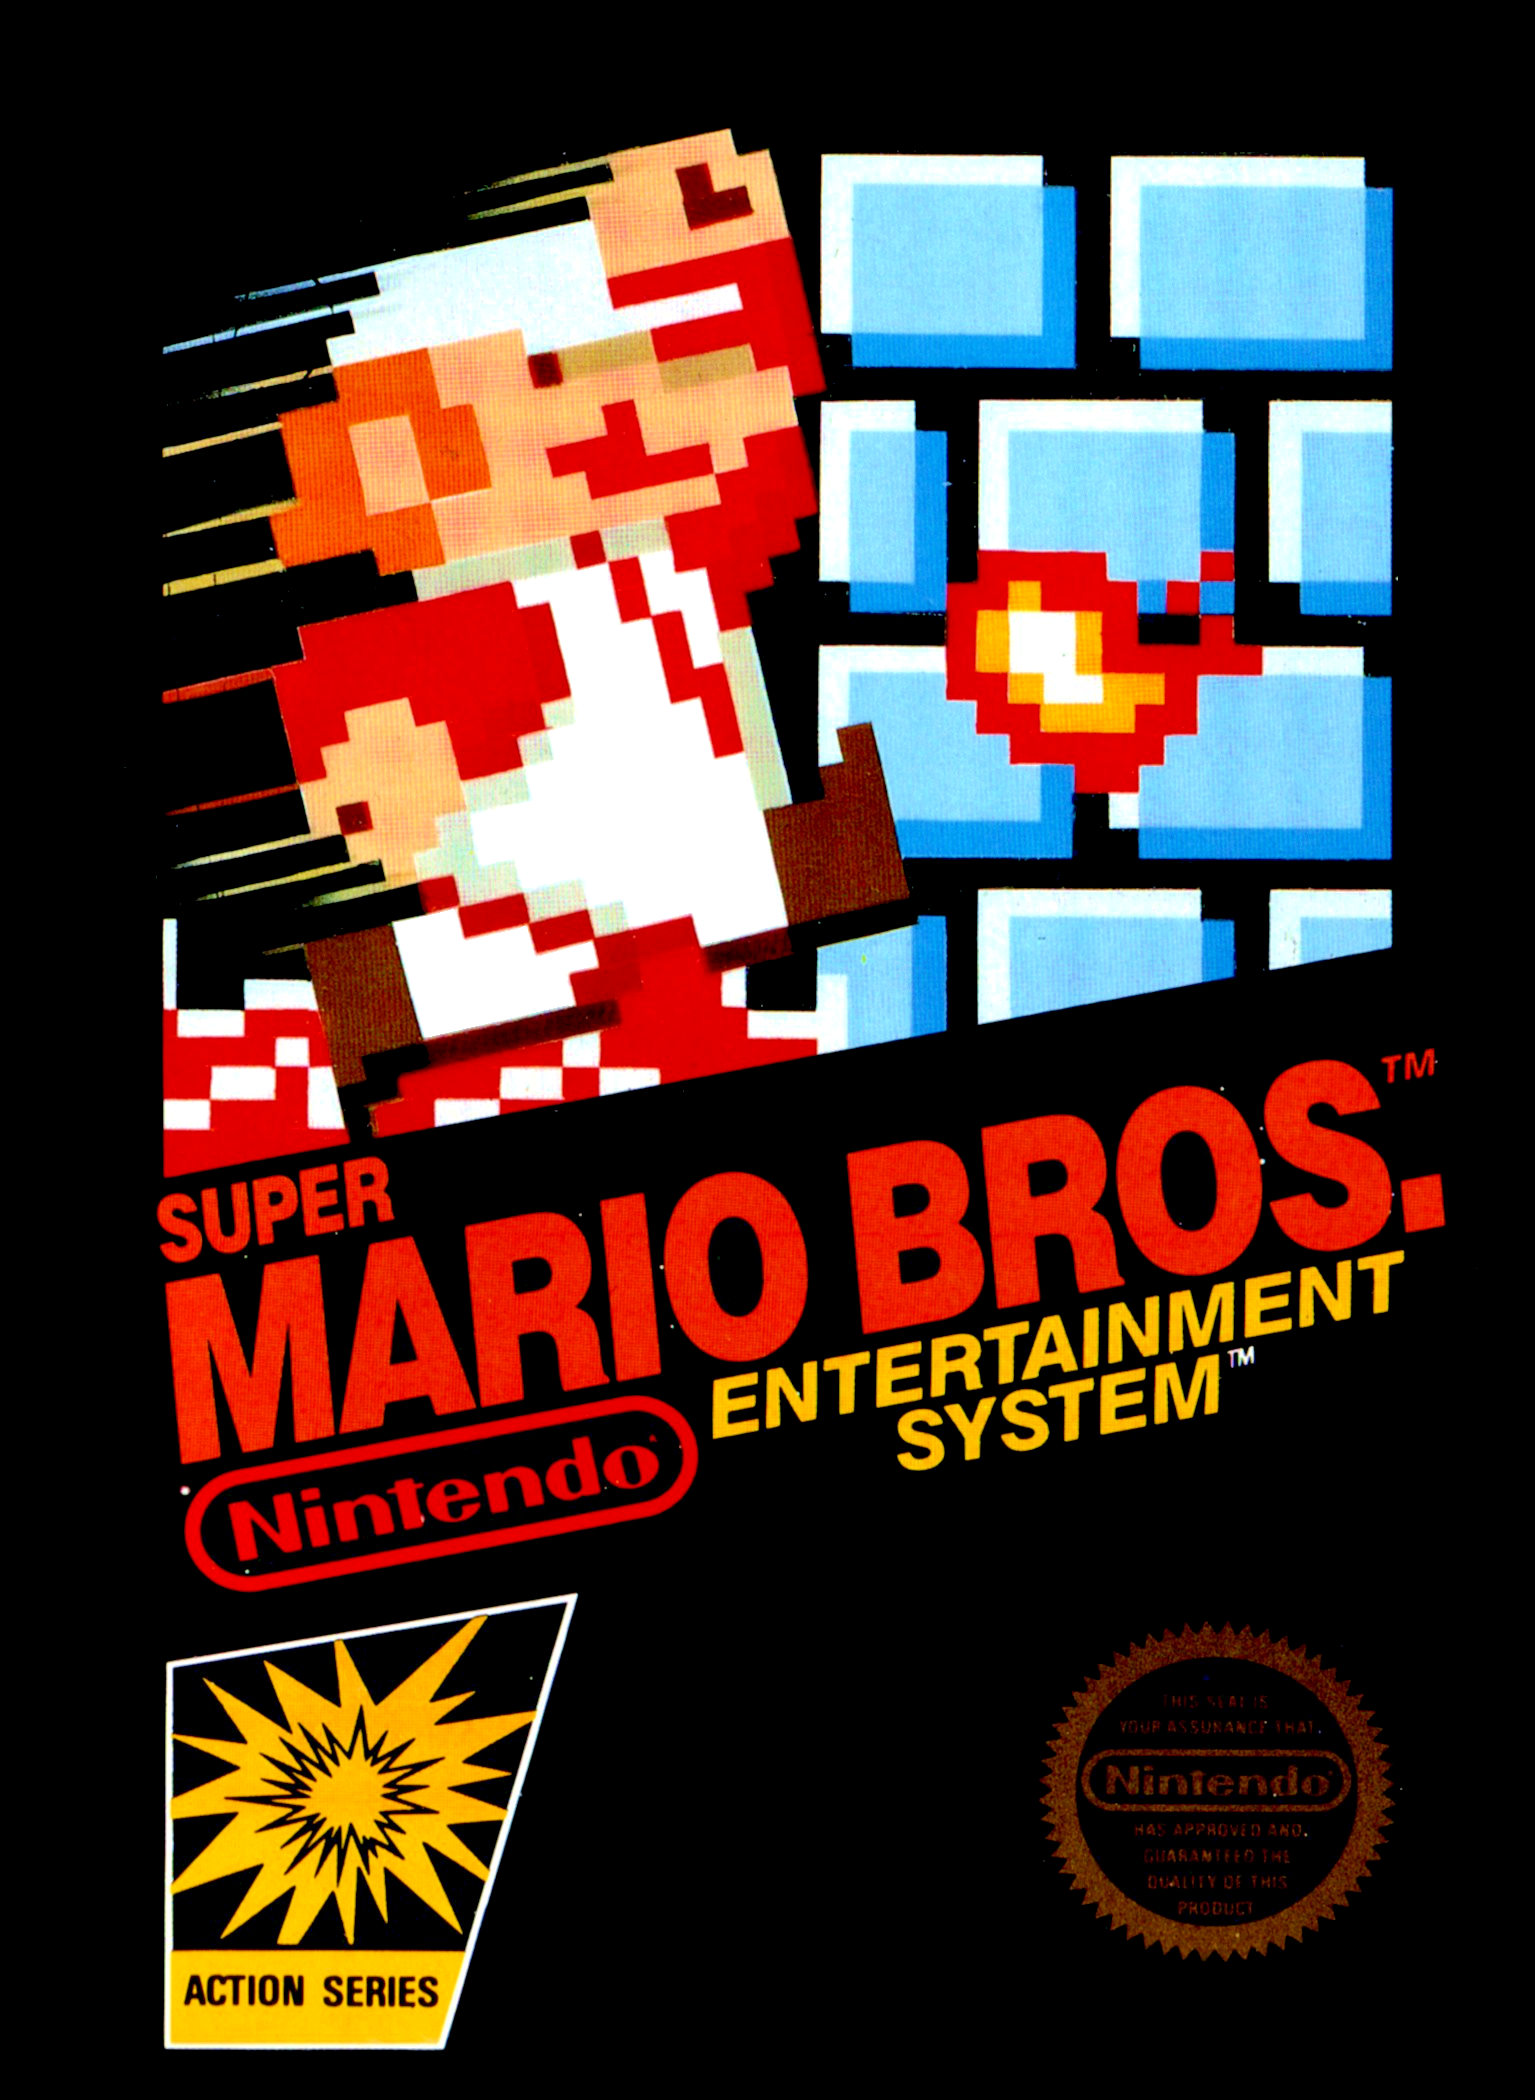
\includegraphics[width=0.4\textwidth]{SMB.png}
                \caption{Jaquette de Super Mario Bros sur NES}
                \label{fig:mesh1}
            \end{figure}

            \newpage

            \begin{figure}[h]
                \centering
                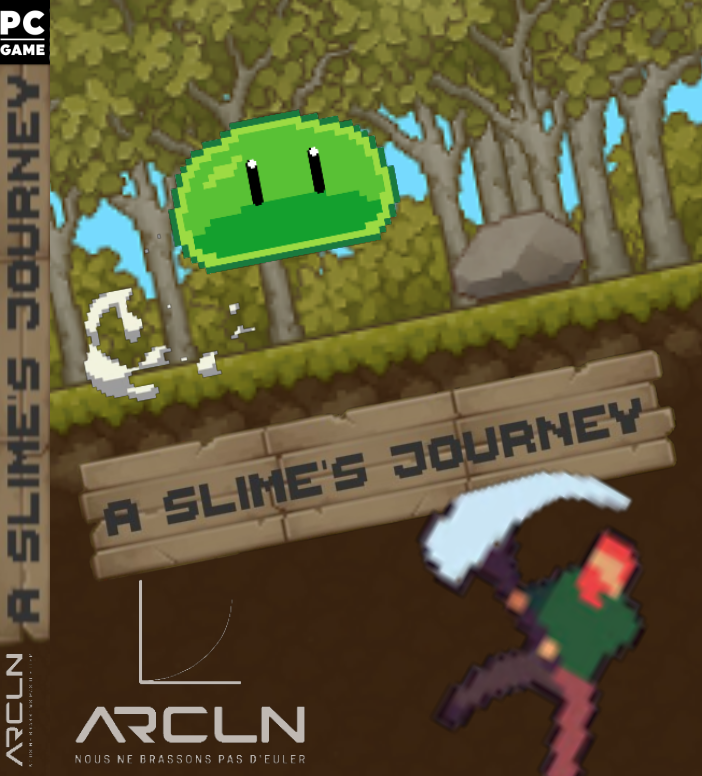
\includegraphics[width=0.4\textwidth]{Jaquette0.png}
                \caption{Recto de la jaquette de jeu}
                \label{fig:mesh1}
            \end{figure}

            Sur la reliure de la jaquette, on retrouve le nom de notre jeu, de notre groupe ainsi que le logo des jeux se jouant sur ordinateur.

            Au verso de la jaquette on peut y trouver une description de “A Slime’s journey” ainsi que des images du niveau un et deux et du logo de l’EPITA.

            \begin{figure}[h]
                \centering
                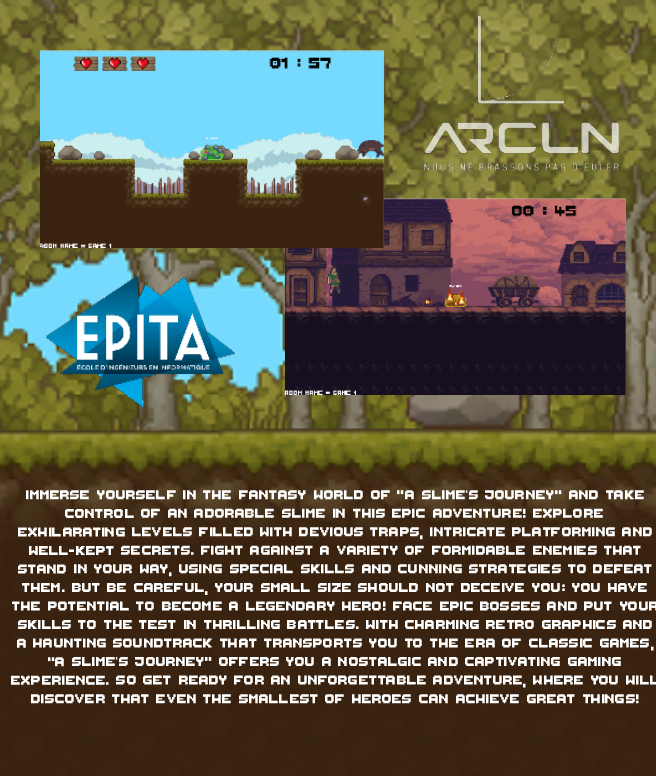
\includegraphics[width=0.4\textwidth]{Jaquette3.png}
                \caption{Verso de la jaquette de jeu}
                \label{fig:mesh1}
            \end{figure}
        \end{indt}

        \newpage

        \begin{indt}{\subsection{Installeur}}
            Afin de créer un installateur correct, nous avons utilisé Inno Setup, un logiciel très connu permettant de créer des installateurs pour nos applications. Nous avons fait le choix de laisser l’utilisateur choisir l’emplacement où il souhaite installer le jeu, cependant, il aura besoin des droits d’administrateur sur son ordinateur afin de procéder à l’installation de “A Slime’s Journey”.
        \end{indt}

        \begin{indt}{\subsection{Répartition des tâches}}
            Pour cette dernière phase du projet, nous avons réalisé une répartition des tâches efficace afin de finaliser avec succès le développement de notre jeu de plateforme, "A Slime's Journey". Chaque membre de l'équipe a contribué de manière significative à différents aspects du jeu, démontrant ainsi notre collaboration et notre engagement collectif.

            Omid s'est investi dans la mise en place de l'IA, apportant des comportements intelligents aux ennemis et aux personnages non joueurs, ce qui a enrichi l'expérience de jeu globale. Alexis s'est consacré à la capacité de transformation du personnage principal, offrant aux joueurs une expérience de jeu dynamique et divertissante. Enzo et Maxime ont assumé la responsabilité de la transformation du personnage et ont également créé un objet spécial qui permet aux joueurs de terminer le niveau et de progresser vers les futurs niveaux lorsque ceux-ci seront disponibles.

            Cette répartition des tâches a favorisé une collaboration étroite entre les membres de l'équipe, permettant ainsi une communication fluide et un partage de connaissances constant. Nous nous sommes mutuellement soutenus, partageant des idées, des conseils et des ressources pour garantir que chaque aspect du jeu atteigne les standards de qualité que nous nous étions fixés.

            De plus, nous avons finalisé le site internet du jeu, veillant à ce qu'il reflète l'identité visuelle et l'ambiance du jeu. En utilisant des captures d'écran du jeu, nous avons personnalisé la page internet, créant ainsi une immersion supplémentaire pour les visiteurs. Sur cette page, nous avons inclus des liens de téléchargement pour le cahier des charges et le dernier rapport de soutenance, offrant ainsi aux intéressés un accès facile à toutes les informations importantes concernant notre projet.

            Et grâce à une répartition efficace des tâches et à notre engagement commun, nous avons réussi à achever le développement de "A Slime's Journey" avec succès. Nous sommes fiers du travail accompli par chaque membre de l'équipe et nous sommes confiants que notre jeu de plateforme offrira une expérience mémorable aux joueurs.
        \end{indt}

        \newpage

        \begin{indt}{\subsection{Site internet}}
            \begin{figure}[h]
                \centering
                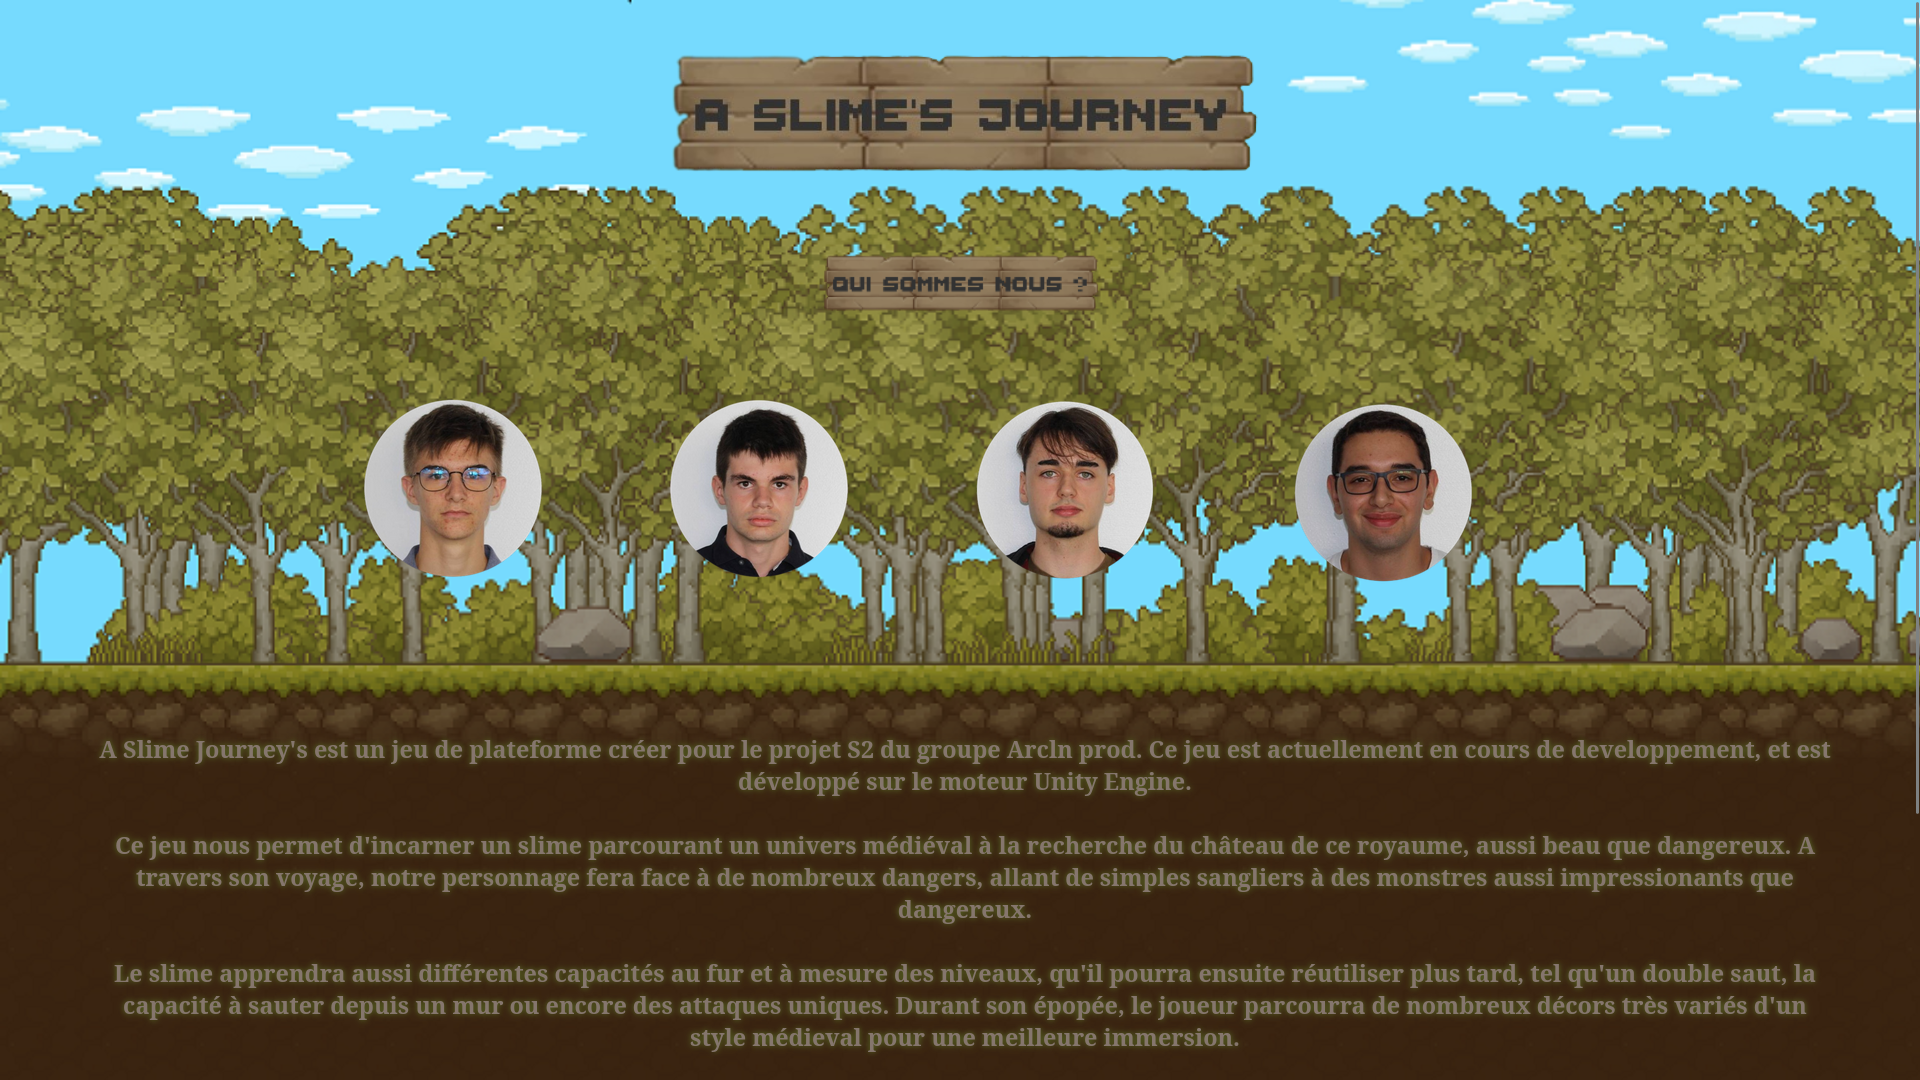
\includegraphics[width=0.6\textwidth]{Site2.png}
                \caption{Site internet du jeu}
                \label{fig:mesh1}
            \end{figure}

            Le site internet à été créé par nous même, en utilisant le HTML, et contient un CSS afin de pouvoir mieux gérer la mise en page du site. Tout d’abord, la création du site en lui-même, en passant par l’application bloc-note afin de savoir ce qui était important de mettre sur le site internet.

            Ensuite, viennent les idées, tel que la mise en arrière plan d’une capture d’écran de notre premier niveau, indiquant le titre du jeu affiché sur une pancarte du menu du jeu, afin de montrer clairement la direction artistique du jeu. L’affichage de l’arrière-plan fut problématique, en effet, l’image n'était pas assez grande, par conséquent, les commandes habituelles afin de faire un arrière-plan qui couvre toute la page était impossible. Après plusieurs essais non concluants, la décision d'agrandir la partie intéressante de l’image à été prise, afin de contourner notre problème. Nous avons également changé l'icône du site pour un slime afin que ce site soit encore plus personnalisé.

            De plus, nous avons intégré nos visages à la rubrique “Qui sommes nous ?”, qui, lorsqu’on passe le curseur dessus affiche une pop-up avec notre rôle au sein du groupe ainsi qu’une rapide présentation.

            Enfin, les liens permettant le téléchargement des documents comme le cahier des charges du projet ainsi que le rapport de la dernière soutenance du projet ont été ajoutés, ainsi qu’un bouton pour pouvoir télécharger l’installateur qui vous permettra de tester notre jeu.
        \end{indt}

        \newpage

        \begin{indt}{\subsection{Planning}}
            La répartition des tâches est un élément essentiel dans le développement d'un projet, et cela s'applique également à notre jeu vidéo "A Slime's Journey" tout au long des trois soutenances. En répartissant les responsabilités entre les membres de l'équipe lors de chaque étape du projet, nous avons pu travailler de manière efficace et coordonnée, en maximisant nos ressources et en garantissant une progression constante.

            Avant la première soutenance, nous avons établi une répartition des tâches claire. Omid s'est concentré sur l'IA, Alexis a travaillé sur la capacité de transformation, Enzo a pris en charge la création du premier niveau, tandis que Maxime s'est chargé du multijoueur et de développer un site web présentant le jeu Cette approche nous a permis de nous spécialiser dans nos domaines respectifs et de progresser de manière efficace, tout en ayant une bonne communication entre nous.

            Pour la deuxième soutenance, nous avons maintenu cette répartition des tâches, tout en ajoutant de nouveaux éléments au jeu. Omid a continué à peaufiner l'IA, Alexis a travaillé sur une nouvelle transformation, le slime de roche, avec un système d'escalade innovant. Enzo a créé le second niveau, tandis que Maxime s'est occupé de développer un prototype de projectile et a ajouté de nouveaux monstres, tels que le Villageois et l'Archer. Cette répartition des tâches nous a permis de progresser rapidement et d'apporter de nouvelles fonctionnalités intéressantes au jeu.

            Enfin, lors de la troisième soutenance, nous avons continué à nous appuyer sur notre répartition des tâches établie précédemment. Omid a travaillé sur la création du boss final, Alexis a ajouté le Slime de feu avec son propre projectile, Enzo s'est occupé des options du jeu, telles que les paramètres de touches, la résolution et le volume sonore, tandis que Maxime a finalisé la création du menu principal. Cette répartition des tâches nous a permis de conclure le projet avec succès, en ajoutant des éléments clés qui améliorent l'expérience de jeu globale.

            En résumé, la répartition des tâches tout au long des trois soutenances de développement de "A Slime's Journey" a joué un rôle crucial dans notre succès. Elle nous a permis d'exploiter les compétences spécifiques de chaque membre de l'équipe, de maintenir une bonne communication et de progresser de manière efficace. Grâce à cette approche, nous avons pu créer un jeu vidéo complet et engageant, en mettant en valeur le talent et la contribution de chaque membre de l'équipe.

            \begin{center}
                \begin{tabular}{|c|l|l|l|}
                    \hline
                    & Première Soutenance & Deuxième soutenance & Troisième soutenance
                    \\
                    \hline
                    Développement
                    & \begin{tabular}{l}
                        $\bullet$ 1 niveau
                        \\
                        $\bullet$ Interactions basiques
                        \\
                        $\bullet$ 1 transformation
                    \end{tabular}
                    & \begin{tabular}{l}
                        $\bullet$ Second niveau
                        \\
                        $\bullet$ Nouvelle forme
                    \end{tabular}
                    & \begin{tabular}{l}
                        $\bullet$ Ajout dernier niveau
                        \\
                        $\bullet$ Ajout de boss
                        \\
                        $\bullet$ Mode boss rush
                    \end{tabular}
                    \\
                    \hline
                    Communication
                    & \begin{tabular}{l}
                        $\bullet$ Site Web
                    \end{tabular}
                    & \begin{tabular}{l}
                        $\bullet$ Réseaux sociaux
                    \end{tabular}
                    & \begin{tabular}{l}
                        $\bullet$ Sortie officielle du jeu
                    \end{tabular}
                    \\
                    \hline
                    Design
                    & \begin{tabular}{l}
                        $\bullet$ Niveau
                        \\
                        $\bullet$ Éléments du décor
                    \end{tabular}
                    & \begin{tabular}{l}
                        $\bullet$ Nouveau niveau
                        \\
                        $\bullet$ Créatures
                    \end{tabular}
                    & \begin{tabular}{l}
                        $\bullet$ Design final du jeu
                    \end{tabular}
                    \\
                    \hline
                    Audio
                    & \begin{tabular}{l}
                        $\bullet$ Musique du niveau
                    \end{tabular}
                    & \begin{tabular}{l}
                        $\bullet$ Nouvelles musiques
                    \end{tabular}
                    & \begin{tabular}{l}
                        $\bullet$ Musiques finales
                    \end{tabular}
                    \\
                    \hline
                    IA
                    & \begin{tabular}{l}
                        $\bullet$ Monstres doté d'une IA
                    \end{tabular}
                    & \begin{tabular}{l}
                        $\bullet$ Différentes IA
                    \end{tabular}
                    & \begin{tabular}{l}
                        $\bullet$ Nouveaux ennemis
                        \\
                        $\bullet$ Nouveaux boss
                    \end{tabular}
                    \\
                    \hline
                    Réseau
                    & \begin{tabular}{l}
                        $\bullet$ Multijoueur en place
                    \end{tabular}
                    & \begin{tabular}{l}
                        $\bullet$ Corrections de bugs
                    \end{tabular}
                    & \begin{tabular}{l}
                        $\bullet$ Mode Versus
                    \end{tabular}
                    \\
                    \hline
                    Rédaction
                    & \begin{tabular}{l}
                        $\bullet$ Cahier des charges
                    \end{tabular}
                    & \begin{tabular}{l}
                        $\bullet$ Nouveau cahier
                        \\
                        des charges
                    \end{tabular}
                    & \begin{tabular}{l}
                        $\bullet$ Rapport du projet
                        \\
                        $\bullet$ Annexes
                        \\
                        $\bullet$ Dossier d'exploitation
                    \end{tabular}
                    \\
                    \hline
                \end{tabular}
            \end{center}
        \end{indt}

        \begin{indt}{\subsection{Projets futur}}
            Si le développement du jeu "A Slime's Journey" se poursuit au-delà de la troisième soutenance, plusieurs nouveautés passionnantes pourraient être envisagées pour enrichir davantage l'expérience de jeu. Tout d'abord, l'introduction de nouveaux niveaux avec des environnements variés offriraient aux joueurs une plus grande diversité de défis et de découvertes. Imaginez un niveau situé dans une forêt mystérieuse avec des plateformes mobiles et des ennemis rusés, ou un niveau souterrain rempli de pièges mortels et de trésors cachés. Ces nouveaux niveaux permettraient d'explorer des mondes encore inconnus, tout en offrant des obstacles et des énigmes uniques à résoudre.

            Ensuite, l'ajout de nouvelles transformations pour notre protagoniste slime serait une idée captivante. Chaque transformation apporterait des capacités spéciales uniques, ouvrant de nouvelles possibilités de gameplay et encourageant les joueurs à adopter des approches différentes pour surmonter les défis. Par exemple, une transformation en slime gelatinux pourrait permettre au joueur de se faufiler à travers de petites ouvertures, tandis qu'une transformation en slime sauteur donnerait au joueur la capacité de réaliser de grands bonds pour atteindre des plateformes éloignées. Ces nouvelles formes de slime apporteraient une dimension supplémentaire à l'exploration et à la résolution des énigmes, offrant une expérience plus riche et stimulante.

            En termes de fonctionnalités, la mise en place d'un éditeur de niveaux intégré serait une idée passionnante pour impliquer davantage la communauté de joueurs. Un tel outil permettrait aux joueurs de créer leurs propres niveaux personnalisés, de les partager avec d'autres joueurs et de les jouer. Cela créerait une expérience de jeu infiniment extensible et favoriserait l'interaction entre les joueurs, stimulant ainsi la créativité et la communauté autour du jeu. De plus, l'intégration de classements en ligne et de défis spéciaux dans les niveaux créés par les joueurs ajouterait une dimension compétitive et inciterait les joueurs à relever de nouveaux défis pour obtenir les meilleurs scores.

            En somme, si le développement de "A Slime's Journey" se poursuit après la troisième soutenance, l'introduction de nouveaux niveaux, de nouvelles transformations et d'un éditeur de niveaux intégré ouvrirait de nouvelles perspectives passionnantes pour les joueurs. Ces ajouts enrichiraient l'expérience de jeu en offrant des défis variés, une exploration approfondie et une interaction communautaire. En s'appuyant sur les fondations solides déjà établies, ces nouveautés permettraient de prolonger la durée de vie du jeu, de susciter l'intérêt des joueurs et de créer une expérience encore plus gratifiante et immersive pour tous les amateurs de jeux de plateforme.
        \end{indt}

        \begin{indt}{\subsection{Post-mortem}}
           Ce projet nous a permis à tous de mettre un pied dans la création de jeux vidéo. Nous avons également appris à travailler efficacement en équipe tout en se servant d’outils permettant de communiquer et partager notre travail à distance. De plus, nous avons tous appris à nous servir de Unity, ainsi qu’à rechercher de nombreuses informations par nous-même. Nous avons tous été très contents de réaliser ce projet en commun, qui nous a permis d’apprendre beaucoup de choses et d'acquérir de nombreuses compétences. En effet, l’utilisation de certains outils comme Git ou encore Unity nous est désormais plus familière.

        \end{indt}
    \end{indt}

    \newpage

    \begin{indt}{\section{Conclusion}}
        L'impression de groupe au sein de notre équipe est extrêmement positive. Nous avons fait d'énormes progrès dans le développement du jeu "A Slime's Journey", et nous sommes fiers de l'atteinte de nos objectifs.

        La partie artistique du jeu est en parfaite adéquation avec notre vision initiale, ce qui témoigne de notre capacité à collaborer et à concrétiser nos idées créatives.
        Un autre point fort est que nous avons résolu tous les problèmes de bugs, ce qui garantit une expérience de jeu fluide et sans accrocs. Nous avons mis en place des procédures rigoureuses de tests et de débogage, ce qui nous a permis de respecter les délais fixés et de livrer un produit de haute qualité.

        En travaillant avec Unity, nous avons tous gagné en compétences et en confiance dans l'utilisation de l'outil. Cela nous a permis de résoudre de nombreux problèmes de manière autonome, ce qui a considérablement accéléré notre progression et nous a fait gagner un temps précieux.
        La communication au sein de notre équipe a été exemplaire. Nous avons maintenu une ligne de communication ouverte, échangeant régulièrement des idées, des suggestions et des mises à jour sur l'avancement du projet. Cette communication efficace a favorisé une collaboration harmonieuse et une meilleure compréhension mutuelle de nos objectifs communs.

        Cependant, nous sommes conscients qu'il reste encore quelques problèmes à résoudre. Nous sommes déterminés à les aborder de front et à les résoudre dans les plus brefs délais, afin de garantir une expérience de jeu optimale pour nos futurs joueurs. Nous sommes confiants dans notre capacité à relever ces défis restants et à améliorer encore davantage notre jeu.

        Dans l'ensemble, nous sommes extrêmement satisfaits de notre progression et de notre travail en équipe. Nous avons surmonté de nombreux obstacles et nous avons réussi à créer un jeu de plateforme captivant et divertissant. Avec notre engagement collectif et notre détermination à relever les défis restants, nous sommes convaincus que "A Slime's Journey" sera un succès remarquable.

        \begin{indt}{\subsection{Enzo}}
            Ce projet a été une expérience incroyablement enrichissante. J'ai ressenti une grande satisfaction en voyant les progrès que nous avons réalisés tout au long du développement. Il y avait énormément de travail à accomplir, mais cela nous a permis de repousser nos limites et de nous dépasser. J'ai également beaucoup apprécié notre veille technique constante, qui nous a permis de rester à la pointe des dernières avancées dans le domaine du jeu vidéo.

            La correction des bugs a été une partie essentielle du processus, mais elle nous a permis d'améliorer la jouabilité et de garantir une expérience fluide pour les joueurs. C'était un défi passionnant de trouver des solutions créatives aux problèmes rencontrés.

            Ce projet a été particulièrement intéressant, car c'était la première fois que nous utilisions une API, en l'occurrence Photon, pour développer un jeu en ligne. Cela nous a permis d'explorer de nouvelles fonctionnalités et d'offrir aux joueurs une expérience multijoueur immersive.

            De plus, "A Slime's Journey" était notre premier projet d'une durée aussi longue. Travailler sur un projet sur le long terme nous a permis de comprendre l'importance de la planification, de la gestion du temps et de la collaboration au sein de l'équipe. Nous avons appris à nous soutenir mutuellement et à tirer le meilleur parti des compétences de chacun.

            En bref, ce jeu a été une aventure passionnante qui m'a permis de grandir en tant que développeur de jeux vidéo. J'ai apprécié la satisfaction de voir le projet avancer, la recherche technique constante, la correction des bugs, ainsi que l'intérêt et l'implication de toute l'équipe. Ce fut une expérience inoubliable de travailler ensemble sur un projet aussi ambitieux.

        \end{indt}

        \begin{indt}{\subsection{Alexis}}
            Ce projet a été une expérience extrêmement gratifiante et unique pour moi. Jusqu'à présent, je n'avais jamais participé à un projet de groupe aussi complet et de longue durée. En plus d'acquérir de nouvelles compétences sur Unity, j'ai surtout appris énormément sur la gestion de projets étalés sur plusieurs mois. La clé de notre réussite résidait dans notre coordination et notre communication régulière au sein du groupe. Nous avons utilisé des outils tels que Git et Github Desktop pour nos commits, et nous nous sommes mutuellement aidés lors du développement du mode multijoueur ainsi qu'au début du projet, lorsque personne ne connaissait rien. Nous avons également consacré beaucoup de temps au débogage intensif avant chaque présentation.

            J'ai également appris à rédiger un cahier des charges, qui s'est révélé essentiel pour faire progresser le projet, ainsi que les rapports de soutenance. Mettre par écrit tout ce que nous avions accompli n'a pas toujours été facile, surtout lorsque nous nous y prenions deux jours avant la présentation en sous-estimant le temps nécessaire. Bien sûr, cela m'a également permis d'apprendre à présenter un travail d'une telle envergure à l'oral et en groupe.

            En fin de compte, malgré le temps et les efforts considérables que ce projet a exigés, j'ai pris plaisir à y travailler car il était enrichissant, créatif et surtout conçu entièrement par notre groupe.
        \end{indt}

        \newpage

        \begin{indt}{\subsection{Omid}}
            Ce projet a été pour moi une expérience très enrichissante et unique.

            Je n’avais jusque là jamais travaillé sur un projet de groupe si complet et d’une aussi longue durée. En dehors de toutes les compétences que j’ai débloquées sur Unity, j’ai surtout apprit de nombreuses choses sur le gestion de projets sur plusieurs mois. En effet, je pense que la clé de notre réussite dans ce projet a été notre coordination et la communication régulière dans le groupe. Que ce soit au niveau des commits et de git (avec la découverte de ce superbe outil qu’est Github Desktop) mais aussi de l’entraide entre tous les membres du groupe notamment dans le développement du multijoueur ou lors des débuts du projet où personne n’y connaissait rien ou encore lors du débuggage intensif avant chaque soutenance.

            J’ai aussi pu apprendre comment rédiger un cahier des charges (qui a été primordial pour la progression du projet) ainsi que les rapports de soutenances. Mettre en texte tout ce que l’on avait fait n’a pas toujours été une tâche facile surtout lorsque l’on s’y prenait deux jours avant la soutenance en sous-estimant le temps que cela prendrait. Bien évidemment, cela m’a aussi permis d’apprendre comment présenter un travail d’une telle ampleur à l’oral et en groupe.

            Finalement, bien que ce projet ait demandé beaucoup de temps et d’efforts, c’était avec plaisir que je travaillais dessus car il était enrichissant, créatif et surtout fait de toutes pièces par notre groupe.
        \end{indt}

        \begin{indt}{\subsection{Maxime}}
            J’ai pris énormément de plaisir à travailler en groupe, sur un sujet de notre choix, tout en menant le projet à bien de A à Z. Nous avons tous su travailler  en équipe, en communiquant tout le temps entre nous, débattant de nos différentes idées pour ce jeu, dont nous sommes aujourd’hui tous fiers. De plus, j’ai acquis de nombreuses compétences comme l’utilisation d’Unity et de Git. J’ai également appris à répartir le travail dans un groupe ainsi qu’à travailler en équipe, avançant tous dans la même direction.. N’ayant pas eu d’architecte au sein du groupe, nous manquons encore un peu d’expérience (trop peu de commentaires dans notre code commun, une architecture qui laisse à désirer), c’est pourquoi si je devais refaire un projet dans le même genre, j'essaierai de commenter plus régulièrement mon code.

            Hors programmation, j’ai aussi découvert l’expérience de la soutenance, en effet, je n’avais jamais défendu un projet personnel aussi important devant un jury. La rédaction de rapport de soutenance et de cahier des charges est également quelque chose de nouveau pour moi, j’ai grandement apprécié cette expérience, en grande partie grâce à notre groupe, qui est très soudé et motivé.
        \end{indt}
    \end{indt}

    \newpage

    \begin{indt}{\section{Bibliographie}}

        \begin{indt}{\subsection{Jeu Vidéo}}
            Unity Asset Store : \href{url}{https://assetstore.unity.com}

            Musique : \href{url}{https://assetstore.unity.com/packages/audio/music/fantasy-rpg-adventure-25-tracks-181574}

            Sprites du slime : \href{url}{https://assetstore.unity.com/packages/2d/characters/slime-enemy-pixel-art-228568}

            Décors : \href{url}{https://assetstore.unity.com/packages/2d/environments/pixel-art-platformer-village-props-166114}

            Multijoueur : \href{url}{https://www.youtube.com/@divingsquid}

            %Déplacement du joueur et création du niveau : \href{url}{https://www.youtube.com/watch?v=Y3-iYIs16TI&list=PLUWxWDlz8PYKnrd27LTqOxL2lr3KhEVRT}

        \end{indt}

        \begin{indt}{\subsection{Communication}}
            Instagram : \href{url}{https://www.instagram.com/arcln$\_$prod}

            Discord : \href{url}{https://discord.gg/nGX33pxS}
        \end{indt}
    \end{indt}

\end{document}
%--------------------------------------------End
